% Πρόβλεψη κίνησης κινητού δικτύου
% Build: xelatex slides.tex (run twice), or: tectonic slides.tex
% Data for the charts: python presentation/export_data.py (raw data, from the repo root)
%                      %run -i presentation/slide_figures.py (forecasts, last cell of the notebook)
%                      Until that has run, the forecast and interval slides fall back to PNGs from the notebook.
% Speaker notes: uncomment the \setbeameroption line below to get slides + notes side by side.
%
% Order follows the six points of the assignment:
%   1 problem and data | protocol | 2 ARIMA | 3 LSTM | 4 TimesFM | 5 metrics and results | 6 6G | backup
\documentclass[aspectratio=169,10pt]{beamer}

\usetheme{metropolis}
\metroset{sectionpage=none, progressbar=frametitle, numbering=fraction, block=fill}
\usefonttheme{professionalfonts}
% \setbeameroption{show notes on second screen=right}

% ---------- fonts and language ----------
\usepackage{fontspec}
\usepackage{polyglossia}
\setmainlanguage{greek}
\setotherlanguage{english}
\setmainfont{FiraSans}[
  Extension = .otf, UprightFont = *-Book, BoldFont = *-SemiBold,
  ItalicFont = *-BookItalic, BoldItalicFont = *-SemiBoldItalic]
\setsansfont{FiraSans}[
  Extension = .otf, UprightFont = *-Book, BoldFont = *-SemiBold,
  ItalicFont = *-BookItalic, BoldItalicFont = *-SemiBoldItalic]
\setmonofont{FiraMono}[Extension = .otf, UprightFont = *-Regular, BoldFont = *-Medium, Scale = 0.92]
\usepackage{amsmath}
\usepackage{unicode-math}
\setmathfont{FiraMath-Regular.otf}

\usepackage{booktabs}
\usepackage{array}
\usepackage{graphicx}
\usepackage{algpseudocode}
\usepackage{tikz}
\usetikzlibrary{positioning, arrows.meta, decorations.pathreplacing}
\usepackage{pgfplots}
\usepgfplotslibrary{groupplots, fillbetween}
\pgfplotsset{compat=1.18}
\graphicspath{{figs/}}

% ---------- colours ----------
% Rule: colour only ever means a series (same colours as the notebook figures).
% Everything else is neutral: models are told apart by line style and shade, emphasis is weight.
% Flat fills, no borders, no rounded corners.
\definecolor{inet}{HTML}{2A78D6}
\definecolor{sms}{HTML}{EB6834}
\definecolor{calls}{HTML}{1BAF7A}
\definecolor{ink}{HTML}{16202A}
\definecolor{text}{HTML}{2B3640}
\definecolor{paper}{HTML}{F7F8FA}
\definecolor{fillc}{HTML}{E8ECF0}
\definecolor{rule}{HTML}{D5DBE1}
\definecolor{muted}{HTML}{66727F}
\definecolor{quiet}{HTML}{8A96A3}

% Stock metropolis look. One override: alerts are bold dark grey instead of orange,
% because orange already means the SMS series in every chart.
\setbeamercolor{alerted text}{fg=mDarkTeal}
\setbeamerfont{alerted text}{series=\bfseries}
\algrenewcommand{\algorithmiccomment}[1]{\hfill{\footnotesize\textcolor{muted}{// #1}}}

\newcommand{\muted}[1]{\textcolor{muted}{#1}}
\newcommand{\figcap}[1]{\par\vspace{2pt}{\scriptsize\muted{#1}}}
% series names with their colour key, as in the figures
\newcommand{\ser}[2]{\textcolor{#1}{\rule[0.05em]{0.6em}{0.6em}}\,#2}
\newcommand{\sInet}{\ser{inet}{Internet}}
\newcommand{\sSms}{\ser{sms}{SMS}}
\newcommand{\sCalls}{\ser{calls}{Calls}}

% ---------- chart style ----------
\pgfplotsset{deck/.style={
  axis x line*=bottom, axis y line*=left, axis line style={draw=rule}, tick style={draw=rule},
  tick label style={font=\tiny, text=muted}, label style={font=\scriptsize, text=muted},
  /pgf/number format/.cd, 1000 sep={.}, use comma, /pgfplots/.cd,
  legend style={draw=none, fill=none, font=\scriptsize, text=text},
  title style={font=\scriptsize, text=ink, anchor=south west, at={(0,1)}, yshift=-1pt}}}

% ---------- title ----------
\title{Πρόβλεψη κίνησης κινητού δικτύου}
\subtitle{Ένα τετράγωνο του Μιλάνου, δύο μήνες δεδομένων, τρεις οικογένειες μοντέλων}
\author{Παναγιώτης Πολυμέρος, Βασίλης Μυλωνάς}
\institute{Αρχιτεκτονικές Δικτύων Επόμενης Γενιάς, επιβλέπων Γιάννης Λακουμέντας}
\date{}

\begin{document}

% =====================================================================
\maketitle
\note{Καλησπέρα. Θα παρουσιάσουμε την πρόβλεψη κίνησης για ένα τετράγωνο του Μιλάνου, το 5060. Θέλουμε να προβλέψουμε την κίνηση δέκα έως πενήντα λεπτά μπροστά, και να συγκρίνουμε τρεις οικογένειες μοντέλων: ARIMA, LSTM και ένα foundation model, το TimesFM. Η παρουσίαση ακολουθεί τα έξι σημεία της εκφώνησης.}

% #####################################################################
\section{Το πρόβλημα και τα δεδομένα}
% #####################################################################

\begin{frame}{Με πρόβλεψη, το δίκτυο δρα πριν τη συμφόρηση}
  Στα 5G/6G πολλές λειτουργίες του δικτύου είναι λογισμικό, οπότε οι πόροι αλλάζουν δυναμικά.
  Το ερώτημα είναι \alert{πότε} να αλλάξουν: πριν ή αφού φτάσει η ζήτηση.

  \vspace{0.9em}
  \centering
  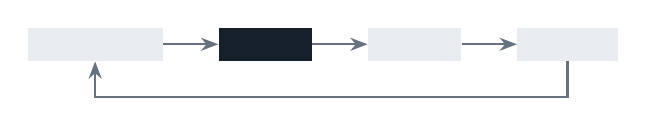
\begin{tikzpicture}[node distance=0.7cm, >={Stealth[length=2.2mm]},
      box/.style={fill=fillc, inner xsep=8pt, inner ysep=6pt, font=\small}]
    \node[box] (m) {παρακολούθηση};
    \node[box, right=of m, fill=ink, text=white, font=\small\bfseries] (a) {ανάλυση};
    \node[box, right=of a] (d) {απόφαση};
    \node[box, right=of d] (e) {εκτέλεση};
    \draw[->, thick, muted] (m) -- (a);
    \draw[->, thick, muted] (a) -- (d);
    \draw[->, thick, muted] (d) -- (e);
    \draw[->, thick, muted] (e.south) -- ++(0,-0.45) -| (m.south);
  \end{tikzpicture}
  \figcap{Ο κλειστός βρόχος του Zero-touch Service Management (ETSI ZSM). Η πρόβλεψη είναι το βήμα της ανάλυσης.}

  \vspace{1em}
  \raggedright
  \begin{columns}[T, onlytextwidth]
    \begin{column}{0.48\textwidth}
      \muted{Short-term, $h = 1$}\\[2pt]
      {\large\textbf{το επόμενο δεκάλεπτο}}\\[2pt]
      \small $\hat y_{t+1}$
    \end{column}
    \begin{column}{0.48\textwidth}
      \muted{Long-term, $H = 5$}\\[2pt]
      {\large\textbf{τα επόμενα πέντε δεκάλεπτα}}\\[2pt]
      \small $\hat y_{t+1}, \dots, \hat y_{t+5}$
    \end{column}
  \end{columns}
  \vspace{0.8em}
  \muted{Αρκετός χρόνος για να ξυπνήσει μια κυψέλη ή να κλιμακωθεί μια εικονική λειτουργία.}
\end{frame}
\note{Το ZSM του ETSI στοχεύει σε δίκτυο που ρυθμίζεται χωρίς ανθρώπινη παρέμβαση, με έναν κλειστό βρόχο: παρακολούθηση, ανάλυση, απόφαση, εκτέλεση. Η πρόβλεψη κίνησης είναι το στάδιο της ανάλυσης· χωρίς αυτήν ο βρόχος αντιδρά αφού έχει ήδη έρθει η συμφόρηση. Με πρόβλεψη μπορεί να δεσμεύσει φάσμα, να ξυπνήσει κυψέλες, να κλιμακώσει εικονικές λειτουργίες ή να μοιράσει χωρητικότητα στα slices πριν φτάσει η ζήτηση. Αντίστροφα, όταν προβλέπεται χαμηλό φορτίο μπορεί να κλείσει εξοπλισμό, αλλά μόνο αν εμπιστευόμαστε την πρόβλεψη. Σε κάθε στιγμή κάνουμε δύο προβλέψεις: το επόμενο δεκάλεπτο και τα πέντε επόμενα.}

% =====================================================================
\begin{frame}{Τα δεδομένα: ένα τετράγωνο στο Duomo, τρεις σειρές}
  \begin{columns}[T, onlytextwidth]
    \begin{column}{0.5\textwidth}
      \small
      \begin{itemize}
        \item Telecom Italia, \emph{Big Data Challenge 2014}: Call Detail Records, 01/11/2013 έως 01/01/2014.
        \item Ένα CDR ανά SMS ή κλήση, και στην αρχή, στο τέλος ή κατά τη διάρκεια μιας σύνδεσης Internet.
        \item Πλέγμα τετραγώνων \textasciitilde 235\,m. Το \alert{5060} είναι πάνω στην Piazza del Duomo.
        \item Ένα σημείο ανά δεκάλεπτο, \alert{χωρίς κανένα κενό}.
      \end{itemize}
    \end{column}
    \begin{column}{0.46\textwidth}
      \small
      \[
        \text{SMS}_t = \text{SMS}^{\text{in}}_t + \text{SMS}^{\text{out}}_t, \qquad
        \text{Calls}_t = \text{Call}^{\text{in}}_t + \text{Call}^{\text{out}}_t
      \]
      \vspace{-0.4em}
      \begin{tabular}{@{}ll@{}}
        \toprule
        Σειρά & Ποιον πόρο φορτώνει \\
        \midrule
        \sInet & User plane: ραδιοπόροι, UPF \\
        \sSms & Σηματοδοσία (AMF, SMSF) \\
        \sCalls & Φωνή με εγγυημένο ρυθμό \\
        \bottomrule
      \end{tabular}
    \end{column}
  \end{columns}
  \vspace{0.5em}
  \begin{block}{Τι πρέπει να έχουμε υπόψη}
    \small Οι τιμές είναι κλιμακωμένες με μια κρυφή σταθερά: \alert{δεν έχουν μονάδα}. Το Internet μετρά εγγραφές, όχι bytes. Ένας μόνο πάροχος, και δεδομένα του 2013, πριν το 5G. \muted{(Barlacchi et al., \emph{Scientific Data}, 2015)}
  \end{block}
\end{frame}
\note{Τα δεδομένα είναι Call Detail Records της Telecom Italia. Για SMS και κλήσεις γράφεται ένα CDR ανά γεγονός. Για το Internet γράφεται όταν ξεκινά ή τελειώνει μια σύνδεση, και ενδιάμεσα αν κρατήσει πάνω από 15 λεπτά ή περάσουν πάνω από 5 MB, οπότε ακολουθεί εν μέρει τον όγκο αλλά δεν είναι ο όγκος. Αθροίζουμε εισερχόμενα και εξερχόμενα, και όλους τους κωδικούς χώρας, γιατί εξυπηρετούνται από τους ίδιους σταθμούς βάσης. Η ανάλυση των δέκα λεπτών δεν αφήνει κανένα κενό και δίνει πάνω από οκτώ χιλιάδες σημεία ανά σειρά, όπως ζητά η εκφώνηση. Οι τιμές είναι κλιμακωμένες με μια κρυφή σταθερά, άρα ένα σφάλμα 50 δεν σημαίνει 50 Mbps ή 50 κλήσεις: τα σφάλματα τα διαβάζουμε σχετικά. Τέλος, η χρήση δεδομένων του 2013 ως εικόνα φορτίου 5G είναι υπόθεση εργασίας της εκφώνησης.}

% =====================================================================
\begin{frame}{Ο ημερήσιος κύκλος κυριαρχεί, οι γιορτές τον σπάνε}
  \begin{columns}[T, onlytextwidth]
    \begin{column}{0.62\textwidth}
      \begin{tikzpicture}
        \begin{groupplot}[deck, group style={group size=1 by 3, vertical sep=0.78cm, xticklabels at=edge bottom},
            width=0.9\linewidth, height=1.15cm, scale only axis, xmin=0, xmax=62, ymin=0,
            xtick={0,9,16,23,30,37,46,53,61}, xticklabels={1/11,10/11,17/11,24/11,1/12,8/12,17/12,24/12,1/1},
            yticklabel style={/pgf/number format/fixed}, ytick distance=500]
          \nextgroupplot[ymax=1700, title={\ser{inet}{Internet}}]
            \addplot[fill=fillc, draw=none, const plot] table[x=x, y expr=\thisrow{off}*1700] {figs/series_hourly.dat} \closedcycle;
            \addplot[inet, line width=0.35pt] table[x=x, y=internet] {figs/series_hourly.dat};
            \draw[ink, dashed] (axis cs:46,0) -- (axis cs:46,1700);
          \nextgroupplot[ymax=1100, title={\ser{sms}{SMS}}]
            \addplot[fill=fillc, draw=none, const plot] table[x=x, y expr=\thisrow{off}*1100] {figs/series_hourly.dat} \closedcycle;
            \addplot[sms, line width=0.35pt] table[x=x, y=sms] {figs/series_hourly.dat};
            \draw[ink, dashed] (axis cs:46,0) -- (axis cs:46,1100);
          \nextgroupplot[ymax=380, ytick distance=150, title={\ser{calls}{Calls}}]
            \addplot[fill=fillc, draw=none, const plot] table[x=x, y expr=\thisrow{off}*380] {figs/series_hourly.dat} \closedcycle;
            \addplot[calls, line width=0.35pt] table[x=x, y=calls] {figs/series_hourly.dat};
            \draw[ink, dashed] (axis cs:46,0) -- (axis cs:46,380);
        \end{groupplot}
      \end{tikzpicture}
      \figcap{Ωριαίος μέσος. Γκρι: Σαββατοκύριακα και αργίες. Διακεκομμένη: αρχή του test.}
    \end{column}
    \begin{column}{0.35\textwidth}
      \small
      \begin{itemize}
        \item Το μεσημέρι το Internet είναι \alert{\textasciitilde 9 φορές} το νυχτερινό.
        \item Το Σαββατοκύριακο SMS και κλήσεις πέφτουν αισθητά, το Internet σχεδόν καθόλου.
        \item Τα Χριστούγεννα η κίνηση πέφτει κάτω από το μισό μιας εργάσιμης, την Πρωτοχρονιά \alert{εκτινάσσεται}.
        \item Καμία τάση. Οι σειρές μοιάζουν μόνο λόγω του κοινού κύκλου: \alert{κάθε σειρά χωριστά}.
      \end{itemize}
    \end{column}
  \end{columns}
\end{frame}
\note{Το πρώτο που φαίνεται είναι ο ημερήσιος κύκλος. Τις καθημερινές η κορυφή είναι γύρω στο μεσημέρι, το Σαββατοκύριακο μετατοπίζεται στο απόγευμα. Τα SMS και οι κλήσεις πέφτουν στο 69 και 55\% μιας εργάσιμης το Σαββατοκύριακο, ενώ το Internet μένει σχεδόν ίδιο, και τη νύχτα του Σαββατοκύριακου είναι πάνω από τριπλάσιο. Τα Χριστούγεννα η κίνηση πέφτει στο 16 έως 39\% μιας εργάσιμης. Στο train οι σειρές έχουν συσχέτιση γύρω στο 0,9, αλλά αν αφαιρέσουμε τον κοινό κύκλο πέφτει στο 0,4, οπότε προβλέπουμε κάθε σειρά μόνη της. Δύο συμπεράσματα για τα μοντέλα: ο τύπος ημέρας αξίζει να δοθεί ως είσοδος, και στις γιορτές του test περιμένουμε μεγαλύτερα σφάλματα.}

% #####################################################################
\section{Πώς αξιολογούμε}
% #####################################################################

\begin{frame}{Μαθαίνουμε στο φθινόπωρο, ελέγχουμε στις γιορτές}
  \centering
  
\begin{tikzpicture}
    \fill[ink]   (0,0) rectangle (9.65,0.75);
    \fill[quiet] (9.65,0) rectangle (13.3,0.75);
    \fill[muted] (8.68,0) rectangle (9.65,0.75);
    \node[anchor=west, text=white, font=\small\bfseries] at (0.25,0.375) {Train, 46 ημέρες};
    \node[anchor=center, text=white, font=\scriptsize] at (9.165,0.375) {valid.};
    \node[anchor=west, text=white, font=\small\bfseries] at (9.85,0.375) {Test, 16 ημέρες};
    \node[anchor=north west, text=muted, font=\scriptsize] at (0,-0.08) {01/11 έως 16/12/2013};
    \node[anchor=north west, text=muted, font=\scriptsize] at (9.65,-0.08) {17/12 έως 01/01};
  \end{tikzpicture}

  \vspace{1.4em}
  \raggedright
  \begin{itemize}
    \item Χωρίζουμε \alert{στον χρόνο}: ένας τυχαίος διαχωρισμός θα έδινε στο μοντέλο τιμές από το μέλλον.
    \item Το test είναι το τελευταίο τέταρτο της σειράς, σε ολόκληρες ημέρες.
    \item Κάθε επιλογή (τάξη, αρχιτεκτονική, ποιο μοντέλο εκπροσωπεί κάθε οικογένεια) γίνεται \alert{μόνο στο train}: στο validation, τις τελευταίες ημέρες του.
    \item Το test πέφτει πάνω σε Χριστούγεννα και Πρωτοχρονιά, που το train δεν έχει δει ποτέ. Αυτό θα αλλάξει ποιο μοντέλο κερδίζει.
  \end{itemize}
\end{frame}
\note{Η εκφώνηση προτείνει 1/3 ή 1/4· κρατάμε το τελευταίο τέταρτο, στρογγυλεμένο σε ολόκληρες ημέρες ώστε το test να ξεκινά στα μεσάνυχτα. Για τα μοντέλα που χρειάζονται επιλογή, LSTM και TimesFM, κρατάμε τις τελευταίες τέσσερις με πέντε ημέρες του train ως validation. Το test δεν χρησιμοποιείται για καμία απόφαση. Επειδή καλύπτει τις γιορτές, ελέγχει και συνθήκες που κανένα μοντέλο δεν έχει δει.}

% =====================================================================
\begin{frame}{Ίδια rolling διαδικασία για κάθε μοντέλο}
  \begin{columns}[T, onlytextwidth]
    \begin{column}{0.42\textwidth}
      \begin{block}{Rolling πρόβλεψη}
        \small
        \begin{algorithmic}
          \State ιστορικό $\gets$ train
          \For{κάθε σημείο $t$ του test}
            \State δώσε στο μοντέλο το ιστορικό
            \State πρόβλεψη $\hat y_{t}, \dots, \hat y_{t+4}$
            \State πρόσθεσε την \textbf{πραγματική} $y_t$
          \EndFor
        \end{algorithmic}
      \end{block}
      \figcap{Siami-Namini et al., ICMLA 2018.}
      \small
      \begin{itemize}
        \item Short-term: το πρώτο βήμα, από κάθε σημείο.
        \item Long-term: και τα πέντε βήματα, από κάθε πέμπτο σημείο, ώστε κάθε τιμή να μετρά μία φορά.
      \end{itemize}
    \end{column}
    \begin{column}{0.54\textwidth}
      \small
      \begin{tabular}{@{}>{\raggedright\arraybackslash}p{0.27\textwidth}>{\raggedright\arraybackslash}p{0.69\textwidth}@{}}
        \toprule
        Μοντέλο & «Δώσε το ιστορικό» σημαίνει \\
        \midrule
        ARIMA-x & νέο fit σε όλο το ιστορικό \\
        LSTM & οι τελευταίες $w$ τιμές ως είσοδος \\
        TimesFM & οι τελευταίες 1024 τιμές ως context \\
        \midrule
        \muted{Naive} & \muted{«όπως τώρα»: $\hat y_{t+j} = y_{t-1}$} \\
        \muted{Seasonal naive} & \muted{«όπως χθες»: $\hat y_{t} = y_{t-144}$} \\
        \bottomrule
      \end{tabular}
      \vspace{0.6em}

      Ένα μοντέλο αξίζει μόνο αν νικά τον κανόνα \alert{«η κίνηση θα μείνει όπως είναι»}.
    \end{column}
  \end{columns}
\end{frame}
\note{Αυτή είναι η τεχνική rolling window του άρθρου των Siami-Namini. Από κάθε σημείο του test προβλέπουμε, και μετά δίνουμε στο μοντέλο την πραγματική τιμή, όπως ένα δίκτυο που μετρά συνεχώς το φορτίο. Η ίδια διαδικασία, ίδια σημεία και ίδιοι ορίζοντες, ισχύει για όλα τα μοντέλα, ώστε η σύγκριση να είναι δίκαιη. Τι σημαίνει «δώσε το ιστορικό» διαφέρει: το ARIMA-x ξαναεκτιμάται κάθε φορά, το LSTM εκπαιδεύεται μία φορά και διαβάζει ένα παράθυρο, το TimesFM διαβάζει ένα μεγάλο context. Μαζί βάζουμε δύο κανόνες που δεν κοστίζουν τίποτα· 144 δεκάλεπτα είναι μία ημέρα. Στα δέκα λεπτά η τελευταία τιμή είναι ήδη πολύ καλή πρόβλεψη, οπότε αυτός είναι ο πραγματικός αντίπαλος.}

% #####################################################################
\section{ARIMA}
% #####################################################################

\begin{frame}{ARIMA: μνήμη των τιμών και μνήμη των λαθών}
  \small
  Με τον τελεστή υστέρησης $B\,y_t = y_{t-1}$ και $\varepsilon_t$ λευκό θόρυβο:
  \vspace{0.3em}

  \begin{columns}[T, onlytextwidth]
    \begin{column}{0.48\textwidth}
      \textbf{AR($p$)}: η τιμή θυμάται πού βρισκόταν
      \[ y_t = c + \phi_1 y_{t-1} + \dots + \phi_p y_{t-p} + \varepsilon_t \]
      \textbf{MA($q$)}: ένα ξάφνιασμα κρατά $q$ βήματα
      \[ y_t = \mu + \varepsilon_t + \theta_1 \varepsilon_{t-1} + \dots + \theta_q \varepsilon_{t-q} \]
    \end{column}
    \begin{column}{0.48\textwidth}
      \textbf{ARIMA($p, d, q$)}: ARMA πάνω στη σειρά διαφορισμένη $d$ φορές
      \[ \phi(B)\,(1 - B)^d\, y_t = c + \theta(B)\,\varepsilon_t \]
      \muted{$\phi(B) = 1 - \phi_1 B - \dots - \phi_p B^p$, \quad $\theta(B) = 1 + \theta_1 B + \dots + \theta_q B^q$}
    \end{column}
  \end{columns}

  \vspace{0.8em}
  \begin{block}{Η προϋπόθεση: στασιμότητα}
    Οι παράμετροι εκτιμώνται στο παρελθόν και εφαρμόζονται στο μέλλον, άρα μέσος, διασπορά και αυτοσυσχέτιση δεν πρέπει να αλλάζουν με τον χρόνο. Η διαφόριση $(1 - B)$ αφαιρεί μια τάση, η εποχική $(1 - B^{s})$ ένα μοτίβο που επαναλαμβάνεται κάθε $s$ βήματα.
  \end{block}
  \vspace{0.3em}
  Τα $d$, $p$, $q$ τα εκτιμούμε \alert{a priori}, με τεστ και γραφήματα.
\end{frame}
\note{Ένα AR λέει ότι η κίνηση τώρα είναι γραμμικός συνδυασμός της κίνησης στα προηγούμενα βήματα: αν είναι υψηλή τώρα, θα είναι μάλλον υψηλή και σε δέκα λεπτά. Ένα MA λέει ότι ένα απρόσμενο γεγονός, π.χ. ένα πλήθος που φτάνει ξαφνικά, επηρεάζει τα επόμενα q βήματα και μετά ξεχνιέται. Το ARIMA εφαρμόζει ARMA στη σειρά αφού τη διαφορίσει d φορές, για να γίνει στάσιμη. Η στασιμότητα είναι η βασική προϋπόθεση, γιατί αλλιώς ό,τι μάθει το μοντέλο στο train δεν ισχύει στο test. Στις επόμενες διαφάνειες βγάζουμε κάθε υπερπαράμετρο από ένα τεστ ή ένα γράφημα.}

% =====================================================================
\begin{frame}{$d = 0$: καμία τάση, αλλά ένας κύκλος που δεν σβήνει}
  \begin{columns}[T, onlytextwidth]
    \begin{column}{0.5\textwidth}
      \small
      \textbf{Τεστ μοναδιαίας ρίζας}, με αντίθετες μηδενικές υποθέσεις:
      \vspace{0.3em}

      \begin{tabular}{@{}lll@{}}
        \toprule
        & H$_0$ & Στη σειρά $y_t$ \\
        \midrule
        ADF & μη στάσιμη & απορρίπτεται, $p \approx 0$ \\
        KPSS & στάσιμη & δεν απορρίπτεται, $p \geq 0{,}1$ \\
        \bottomrule
      \end{tabular}
      \vspace{0.5em}

      Συμφωνούν και στις τρεις σειρές: \alert{καμία τάση, $d = 0$}.
      \vspace{0.6em}

      Τα δύο τεστ όμως δεν βλέπουν την εποχικότητα. Αυτό το δείχνει η ACF: κορυφές \alert{κάθε μέρα την ίδια ώρα}, που σχεδόν δεν μικραίνουν. Χρειάζεται εποχική διαφόριση, \alert{$D = 1$ με $s = 144$}, ή όροι που περιγράφουν τον κύκλο.
    \end{column}
    \begin{column}{0.46\textwidth}
      \begin{tikzpicture}
        \begin{axis}[deck, width=0.92\linewidth, height=3.2cm, scale only axis,
            xmin=0, xmax=3, xtick={0,1,2,3}, xlabel={υστέρηση σε ημέρες},
            ymin=-0.4, ymax=1.05, ytick={0,0.5,1}, yticklabel style={/pgf/number format/use comma},
            title={ACF της $y_t$, Internet}]
          \addplot[ycomb, inet, line width=0.3pt] table[x=lag, y=acf] {figs/acf_y.dat};
          \draw[rule] (axis cs:0,0) -- (axis cs:3,0);
        \end{axis}
      \end{tikzpicture}
      \figcap{Στο train. Ίδια εικόνα στα SMS και Calls.}
    \end{column}
  \end{columns}
\end{frame}
\note{Το ADF έχει μηδενική υπόθεση τη μοναδιαία ρίζα, το KPSS τη στασιμότητα· όταν συμφωνούν, το συμπέρασμα είναι αξιόπιστο. Εδώ το ADF απορρίπτει με p-value πρακτικά μηδέν και το KPSS δεν απορρίπτει, και στις τρεις σειρές, οπότε δεν χρειάζεται απλή διαφόριση. Τα τεστ αυτά όμως κοιτούν μόνο μακροπρόθεσμη τάση και είναι τυφλά σε έναν κύκλο που ανεβοκατεβαίνει κάθε μέρα. Η ACF της σειράς, δεξιά, έχει κορυφή στη μία ημέρα και σχεδόν το ίδιο ύψος στις δύο και τρεις: το ημερήσιο μοτίβο επαναλαμβάνεται σχεδόν ίδιο, και ένα ARMA χαμηλής τάξης δεν μπορεί να το περιγράψει. Γι' αυτό δεν εκτιμούμε καθαρό ARIMA.}

% =====================================================================
\begin{frame}{Μετά τη διαφορά από χθες: τα $p$, $q$, $P$, $Q$}
  \begin{columns}[T, onlytextwidth]
    \begin{column}{0.58\textwidth}
      \begin{tikzpicture}
        \begin{axis}[deck, name=top, width=0.92\linewidth, height=1.35cm, scale only axis,
            xmin=0, xmax=7, xtick={0,1,...,7}, ymin=-0.4, ymax=1.05, ytick={0,0.5,1},
            yticklabel style={/pgf/number format/use comma},
            title={ACF της $y_t - y_{t-144}$, Internet, ως μία εβδομάδα (σε ημέρες)}]
          \addplot[ycomb, inet, line width=0.3pt] table[x=lag, y=acf] {figs/acf_d.dat};
          \draw[rule] (axis cs:0,0) -- (axis cs:7,0);
        \end{axis}
      \end{tikzpicture}

      \vspace{0.35cm}
      \begin{tikzpicture}
        \begin{groupplot}[deck, group style={group size=3 by 1, horizontal sep=0.25cm, yticklabels at=edge left},
            width=0.27\linewidth, height=1.35cm, scale only axis, xmin=0, xmax=36,
            xtick={0,12,24,36}, ymin=-0.2, ymax=1.05, ytick={0,0.5,1},
            yticklabel style={/pgf/number format/use comma}]
          \nextgroupplot[title={PACF, \sInet}]
            \fill[fillc] (axis cs:0,-0.0243) rectangle (axis cs:36,0.0243);
            \addplot[ycomb, inet, line width=0.5pt] table[x=lag, y=internet] {figs/pacf_d.dat};
          \nextgroupplot[title={\sSms}]
            \fill[fillc] (axis cs:0,-0.0243) rectangle (axis cs:36,0.0243);
            \addplot[ycomb, sms, line width=0.5pt] table[x=lag, y=sms] {figs/pacf_d.dat};
          \nextgroupplot[title={\sCalls}]
            \fill[fillc] (axis cs:0,-0.0243) rectangle (axis cs:36,0.0243);
            \addplot[ycomb, calls, line width=0.5pt] table[x=lag, y=calls] {figs/pacf_d.dat};
        \end{groupplot}
      \end{tikzpicture}
      \figcap{Κάτω: PACF της ίδιας σειράς, υστέρηση σε δεκάλεπτα. Γκρι ζώνη: ό,τι θα έβγαινε από τύχη (95\%). Όλα στο train.}
    \end{column}
    \begin{column}{0.39\textwidth}
      \small
      \begin{itemize}
        \item \textbf{Αρνητική ακίδα στη 1 ημέρα}, τίποτα στις 2, 3: εποχικό MA, \alert{$P = 0$, $Q = 1$}.
        \item \textbf{Κορυφή στις 7 ημέρες}: εβδομαδιαίο μοτίβο, που ένα SARIMA ημέρας δεν πιάνει.
        \item \textbf{PACF}: μεγάλη στα πρώτα 4–6 δεκάλεπτα και μετά σχεδόν μηδέν, ενώ η ACF φθίνει: \alert{AR με $p \approx 4$–$6$}, ή ένα μικρό ARMA.
        \item Την τελική τάξη τη διαλέγει το \alert{BIC}.
      \end{itemize}
    \end{column}
  \end{columns}
\end{frame}
\note{Αφαιρούμε την τιμή της ίδιας ώρας χθες και ξανακοιτάμε. Πάνω, η ACF ως μία εβδομάδα: μια αρνητική ακίδα ακριβώς στη μία ημέρα και τίποτα σταδιακό στις επόμενες, που είναι η υπογραφή ενός εποχικού MA πρώτης τάξης. Υπάρχει και μια μεγάλη κορυφή στις επτά ημέρες: η άνοδος της Δευτέρας και η πτώση του Σαββάτου επαναλαμβάνονται κάθε εβδομάδα. Ένα SARIMA με περίοδο την ημέρα δεν μπορεί να την περιγράψει, και με περίοδο την εβδομάδα δεν είναι πρακτικά εφικτό. Κάτω, η PACF για τα πρώτα 36 δεκάλεπτα και στις τρεις σειρές: λίγες μεγάλες τιμές στην αρχή και μετά σχεδόν μηδέν, ενώ η ACF φθίνει σταδιακά. Κατά Box-Jenkins αυτό είναι ένα AR. Επειδή η PACF δεν κόβεται απότομα, δοκιμάζουμε και μικρά ARMA και αφήνουμε το BIC να διαλέξει.}

% =====================================================================
\begin{frame}{Δύο τρόποι να δώσουμε τον κύκλο στο ARIMA}
  \begin{columns}[T, onlytextwidth]
    \begin{column}{0.48\textwidth}
      \begin{block}{SARIMA$(p,0,q)(0,1,1)_{144}$}
        \small
        \[ \phi(B)\,(1 - B^{144})\, y_t = \theta(B)\,(1 + \Theta_1 B^{144})\,\varepsilon_t \]
        Μοντελοποιεί τη διαφορά από \alert{χθες την ίδια ώρα}.
      \end{block}
    \end{column}
    \begin{column}{0.48\textwidth}
      \begin{block}{ARIMA-x}
        \small
        \[ y_t = \beta^{\mathrm{T}} x_t + u_t, \qquad \phi(B)\,u_t = \theta(B)\,\varepsilon_t \]
        Ο κύκλος από \alert{γνωστές μεταβλητές} $x_t$: όροι Fourier ημέρας και εβδομάδας, δείκτης αργίας.
      \end{block}
    \end{column}
  \end{columns}
  \vspace{0.7em}
  \begin{columns}[T, onlytextwidth]
    \begin{column}{0.48\textwidth}
      \small
      \begin{tabular}{@{}lcc@{}}
        \toprule
        Τάξη $(p,0,q)$, BIC & SARIMA & ARIMA-x \\
        \midrule
        \sInet & (2,0,1) & (1,0,1) \\
        \sSms & (2,0,1) & (2,0,1) \\
        \sCalls & (6,0,0) & (1,0,1) \\
        \bottomrule
      \end{tabular}
      \figcap{$\text{BIC} = -2\ln L + k \ln n$: προσαρμογή μείον πολυπλοκότητα.}
    \end{column}
    \begin{column}{0.48\textwidth}
      \small
      \begin{itemize}
        \item Οι όροι του ARIMA-x εξηγούν μόνοι τους \alert{\textasciitilde 90\%} της μεταβολής.
        \item Γι' αυτό οι τάξεις βγαίνουν \alert{μικρές}: μένει λίγη μνήμη για το ARMA.
        \item Το $x_t$ είναι γνωστό για κάθε μελλοντική στιγμή, άρα δεν χρειάζεται πρόβλεψη.
      \end{itemize}
    \end{column}
  \end{columns}
\end{frame}
\note{Η εκφώνηση προτείνει δύο παραλλαγές, και τις δοκιμάσαμε και τις δύο. Το SARIMA κάνει την εποχική διαφόριση που έδειξε η ACF, με έναν εποχικό όρο MA. Το ARIMA-x γράφει τη σειρά ως παλινδρόμηση σε δείκτες περιοδικότητας: ημιτονοειδείς όρους με περίοδο την ημέρα και την εβδομάδα, και έναν δείκτη Σαββατοκύριακου ή αργίας, που επιτρέπει στην Κυριακή να έχει άλλο σχήμα από τη Δευτέρα. Το ημερολόγιο είναι γνωστό από πριν, οπότε αυτές οι μεταβλητές δεν χρειάζονται πρόβλεψη. Για κάθε μοντέλο δοκιμάσαμε ένα μικρό πλέγμα γύρω από τις τιμές των γραφημάτων και κρατήσαμε το μικρότερο BIC, που τιμωρεί τις επιπλέον παραμέτρους. Το BIC προσθέτει σχεδόν παντού ένα MA, γιατί ένα μικρό ARMA κάνει τη δουλειά ενός μεγαλύτερου AR.}

% =====================================================================
\begin{frame}{Τα κατάλοιπα είναι σχεδόν θόρυβος, αλλά το SARIMA είναι αργό}
  \begin{columns}[T, onlytextwidth]
    \begin{column}{0.5\textwidth}
      \textbf{Διαγνωστικός έλεγχος στο train}
      \vspace{0.3em}

      \small
      \begin{itemize}
        \item Αυτοσυσχέτιση καταλοίπων \alert{κάτω από 0,1} σε κάθε υστέρηση: η δομή έχει πιαστεί.
        \item \alert{Βαριές ουρές}: λίγες απρόβλεπτες αιχμές.
        \item Τη μέρα τα σφάλματα είναι \alert{μεγαλύτερα} από τη νύχτα. Θα φανεί στα διαστήματα πρόβλεψης.
        \item Στο SARIMA $\Theta_1 \approx -1$: μαθαίνει ένα σταθερό σχήμα ημέρας, την ίδια ιδέα με το Fourier.
      \end{itemize}
    \end{column}
    \begin{column}{0.46\textwidth}
      \textbf{Κόστος ενός fit}
      \vspace{0.5em}

      \begin{tabular}{@{}lr@{}}
        SARIMA & \alert{\large\textasciitilde 22 λεπτά} \\[3pt]
        ARIMA-x & \large\textasciitilde 11 δευτερόλεπτα \\
      \end{tabular}
      \vspace{0.6em}

      \small
      Η rolling διαδικασία θέλει ένα fit ανά σημείο του test: για το SARIMA περίπου \alert{έναν μήνα} ανά σειρά.
      \vspace{0.6em}

      \muted{Στη σύγκριση την οικογένεια ARIMA την εκπροσωπεί το ARIMA-x.}
    \end{column}
  \end{columns}
\end{frame}
\note{Αν το μοντέλο έχει πιάσει τη δομή της σειράς, τα σφάλματα ενός βήματος στο train πρέπει να μοιάζουν με λευκό θόρυβο. Η μεγαλύτερη αυτοσυσχέτιση μένει κάτω από 0,1. Το Ljung-Box απορρίπτει παρ' όλα αυτά σχεδόν παντού, αλλά με χιλιάδες σημεία ανιχνεύει και πολύ μικρές αυτοσυσχετίσεις. Τα κατάλοιπα δεν είναι κανονικά: έχουν βαριές ουρές και είναι μεγαλύτερα τη μέρα, κάτι που επηρεάζει τα διαστήματα πρόβλεψης. Το SARIMA κουβαλά στη μνήμη του μια ολόκληρη ημέρα διαταραχών, οπότε κάθε fit είναι πολύ αργό. Με ένα νέο fit σε κάθε σημείο του test θα χρειαζόταν περίπου έναν μήνα υπολογισμού ανά σειρά, οπότε από εδώ και πέρα συνεχίζουμε μόνο με το ARIMA-x.}

% #####################################################################
\section{LSTM}
% #####################################################################

\begin{frame}{LSTM: ένα αναδρομικό δίκτυο που διαλέγει τι θα θυμάται}
  \begin{columns}[T, onlytextwidth]
    \begin{column}{0.52\textwidth}
      \small
      \vspace{-0.6em}
      \begin{align*}
        f_t &= \sigma(W_f x_t + U_f h_{t-1} + b_f) && \text{\muted{τι ξεχνάμε}} \\
        i_t &= \sigma(W_i x_t + U_i h_{t-1} + b_i) && \text{\muted{τι γράφουμε}} \\
        \tilde c_t &= \tanh(W_c x_t + U_c h_{t-1} + b_c) && \text{\muted{νέα πληροφορία}} \\
        c_t &= f_t \odot c_{t-1} + i_t \odot \tilde c_t && \text{\muted{μνήμη}} \\
        o_t &= \sigma(W_o x_t + U_o h_{t-1} + b_o) && \text{\muted{τι διαβάζουμε}} \\
        h_t &= o_t \odot \tanh(c_t) && \text{\muted{έξοδος}}
      \end{align*}
    \end{column}
    \begin{column}{0.44\textwidth}
      \small
      \begin{itemize}
        \item Διαβάζει την ακολουθία ένα βήμα τη φορά, με τα \alert{ίδια βάρη} σε κάθε βήμα, όπως η ARIMA με τους ίδιους συντελεστές.
        \item Σε ένα απλό RNN το gradient πολλαπλασιάζεται σε κάθε βήμα και \alert{σβήνει}: δεν μαθαίνει τι έγινε μία ημέρα πριν.
        \item Στο LSTM η μνήμη $c_t$ ενημερώνεται \alert{προσθετικά}. Όταν $f_t \approx 1$, πληροφορία και gradient περνούν πολλά βήματα σχεδόν αναλλοίωτα.
        \item Σε αντίθεση με την ARIMA, είναι \alert{μη γραμμικό}.
      \end{itemize}
    \end{column}
  \end{columns}
\end{frame}
\note{Ένα νευρωνικό δίκτυο μαθαίνει μια μη γραμμική συνάρτηση του ιστορικού, οπότε κατ' αρχήν μπορεί να μάθει σχέσεις που η ARIMA δεν εκφράζει. Ένα RNN κρατά μια κρυφή κατάσταση που λειτουργεί σαν μνήμη. Το πρόβλημα είναι ότι στην εκπαίδευση το gradient προς ένα βήμα k θέσεις πίσω είναι γινόμενο k παραγόντων, και αν αυτοί είναι μικρότεροι από ένα, σβήνει εκθετικά. Για εμάς αυτό μετράει, γιατί ένα παράθυρο μιας ημέρας είναι 144 βήματα. Το LSTM προσθέτει μια δεύτερη κατάσταση, τη μνήμη του κελιού, και τρεις πύλες με τιμές από μηδέν έως ένα. Η μνήμη ενημερώνεται με πρόσθεση, οπότε το gradient από βήμα σε βήμα είναι απλώς η πύλη λήθης· όταν το δίκτυο μάθει να την κρατά κοντά στο ένα, θυμάται για πολύ.}

% =====================================================================
\begin{frame}{Πώς ρυθμίσαμε το LSTM}
  \small
  \begin{columns}[T, onlytextwidth]
    \begin{column}{0.48\textwidth}
      \begin{block}{Είσοδος: ένα παράθυρο}
        Οι τελευταίες $w$ τιμές: $w = 10$ (της εκφώνησης) ή $w = 144$ (μία ημέρα). Για το long-term βγάζει \alert{και τις 5 τιμές μαζί}, οπότε ένα λάθος δεν γίνεται είσοδος στο επόμενο βήμα.
      \end{block}
      \begin{block}{Κανονικοποίηση min-max}
        \[ \tilde y_t = \frac{y_t - y_{\min}}{y_{\max} - y_{\min}} \in [0, 1] \]
        και το αντίστροφο στην έξοδο. Τα όρια \alert{μόνο από το train}, αλλιώς θα «ήξερε» την αιχμή της Πρωτοχρονιάς.
      \end{block}
    \end{column}
    \begin{column}{0.48\textwidth}
      \begin{block}{Από-περιοδικοποίηση (προαιρετική)}
        \[ r_t = y_t - S_t \;\longrightarrow\; \text{LSTM} \;\longrightarrow\; \hat y_t = \hat r_t + S_t \]
        $S_t$: η μέση τιμή για τον ίδιο τύπο ημέρας και την ίδια ώρα. Το δίκτυο μαθαίνει μόνο τις αποκλίσεις.
      \end{block}
      \begin{block}{Δίκτυο}
        2 στρώματα, \textasciitilde 50 χιλ. παράμετροι, early stopping στο validation.
      \end{block}
    \end{column}
  \end{columns}
  \vspace{0.3em}
  \alert{24 δίκτυα}: 3 σειρές × 2 παράθυρα × με ή χωρίς από-περιοδικοποίηση × 2 ορίζοντες.
\end{frame}
\note{Σε αντίθεση με την ARIMA, εδώ το παράθυρο είναι πραγματική επιλογή, γιατί το δίκτυο βλέπει μόνο ό,τι είναι μέσα του. Δοκιμάσαμε το παράθυρο της εκφώνησης, 100 λεπτά, και μία ολόκληρη ημέρα. Η κανονικοποίηση χρειάζεται γιατί οι πύλες κορεννύνται με μεγάλες τιμές: με τιμές της τάξης του χιλίου θα κολλούσαν στο μηδέν ή στο ένα. Η από-περιοδικοποίηση είναι η ίδια ιδέα με το ARIMA-x: αφαιρούμε το γνωστό σχήμα της ημέρας και το δίκτυο μαθαίνει μόνο τις αποκλίσεις. Για το μικρό παράθυρο είναι ο μόνος τρόπος να ξέρει ότι σε μία ώρα έρχεται η μεσημεριανή αιχμή. Μπορεί όμως να βλάψει όταν το μέλλον δεν μοιάζει με το παρελθόν, όπως στις γιορτές. Η εκπαίδευση γίνεται με MSE και Adam, και σταματά όταν το validation δεν βελτιώνεται.}

% =====================================================================
\begin{frame}{Στο validation η από-περιοδικοποίηση βοηθά}
  \begin{columns}[T, onlytextwidth]
    \begin{column}{0.57\textwidth}
      \footnotesize
      \begin{tabular}{@{}llcccc@{}}
        \toprule
        & & \multicolumn{2}{c}{$w = 10$} & \multicolumn{2}{c}{$w = 144$} \\
        \cmidrule(lr){3-4}\cmidrule(l){5-6}
        Σειρά & ορίζ. & raw & deseas. & raw & deseas. \\
        \midrule
        \sInet   & 10\,λεπ. & 56,6 & 55,4 & 57,5 & \alert{54,3} \\
                 & 50\,λεπ. & 84,1 & 65,5 & 78,9 & \alert{64,0} \\
        \sSms    & 10\,λεπ. & 20,8 & 18,9 & 19,0 & \alert{18,8} \\
                 & 50\,λεπ. & 25,5 & 19,9 & 21,6 & \alert{19,8} \\
        \sCalls  & 10\,λεπ. & 15,2 & 13,6 & 14,9 & \alert{13,5} \\
                 & 50\,λεπ. & 19,3 & 14,9 & 16,5 & \alert{14,7} \\
        \bottomrule
      \end{tabular}
      \figcap{RMSE στο validation (οι τελευταίες ημέρες του train). Έντονα: το καλύτερο ανά γραμμή.}
    \end{column}
    \begin{column}{0.4\textwidth}
      \small
      \begin{itemize}
        \item Η από-περιοδικοποίηση μειώνει το σφάλμα λίγο στα 10 λεπτά και \alert{αισθητά στα 50}.
        \item Το validation διαλέγει παντού \alert{$w = 144$, με από-περιοδικοποίηση}. Αυτό εκπροσωπεί το LSTM.
        \item Το παράθυρο της ημέρας θέλει \textasciitilde 4 φορές περισσότερη εκπαίδευση.
      \end{itemize}
    \end{column}
  \end{columns}
  \vspace{0.4em}
  \begin{block}{Αλλά}
    Το validation είναι κανονικές μέρες του Δεκεμβρίου. Στο test, με τις γιορτές, η εικόνα αντιστρέφεται.
  \end{block}
\end{frame}
\note{Όλα τα δίκτυα συγκλίνουν, και το early stopping σταματά πολύ πριν από το όριο των εποχών. Στο validation η από-περιοδικοποίηση μειώνει το σφάλμα από 1 έως 11\% στα δέκα λεπτά και από 8 έως 23\% στα πενήντα. Με βάση όσα ξέρουμε πριν το test, το LSTM με παράθυρο μίας ημέρας και από-περιοδικοποίηση είναι η λογική επιλογή, και είναι ο εκπρόσωπος της οικογένειας. Στα αποτελέσματα θα δούμε ότι στις γιορτές η επιλογή αυτή κοστίζει.}

% #####################################################################
\section{TimesFM}
% #####################################################################

\begin{frame}{TimesFM: ένα foundation model για χρονοσειρές}
  \centering
  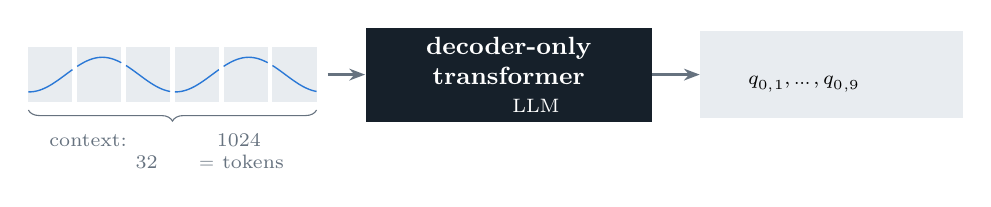
\begin{tikzpicture}[>={Stealth[length=2mm]}]
    % context cut into patches
    \foreach \i in {0,...,5} {
      \fill[fillc] (\i*0.62,0) rectangle (\i*0.62+0.56,0.7);
      \draw[inet, line width=0.5pt, domain=0:0.56, samples=20, smooth]
        plot ({\i*0.62+\x}, {0.35+0.22*sin(deg(2*pi*(\i*0.62+\x)/3.72*2 - 1.6))});
    }
    \draw[decorate, decoration={brace, mirror, amplitude=4pt}, muted] (0,-0.1) -- (3.66,-0.1)
      node[midway, below=5pt, font=\scriptsize, text=muted, align=center] {context: οι τελευταίες 1024 τιμές\\κομμάτια των 32 τιμών $=$ tokens};
    \node[fill=ink, text=white, font=\small\bfseries, minimum height=1.1cm, text width=3.4cm, align=center]
      (tr) at (6.1,0.35) {decoder-only transformer\\[-1pt]{\scriptsize\mdseries όπως ένα LLM}};
    \draw[->, thick, muted] (3.8,0.35) -- (tr.west);
    \node[fill=fillc, font=\small, minimum height=1.1cm, text width=3.1cm, align=center]
      (q) at (10.2,0.35) {ποσοστημόρια\\[-1pt]{\scriptsize $q_{0{,}1}, \dots, q_{0{,}9}$ ανά βήμα}};
    \draw[->, thick, muted] (tr.east) -- (q.west);
  \end{tikzpicture}

  \vspace{1.2em}
  \raggedright
  \begin{columns}[T, onlytextwidth]
    \begin{column}{0.48\textwidth}
      \small
      \begin{itemize}
        \item Προεκπαιδευμένο \alert{μία φορά} από τη Google σε τεράστιο όγκο ετερογενών χρονοσειρών.
        \item Η attention συγκρίνει \alert{άμεσα} το τώρα με την ίδια ώρα πριν από μία εβδομάδα. Το LSTM πρέπει να το κουβαλήσει στη μνήμη του.
      \end{itemize}
    \end{column}
    \begin{column}{0.48\textwidth}
      \small
      \begin{tabular}{@{}lll@{}}
        \toprule
        & ARIMA, LSTM & TimesFM \\
        \midrule
        Γνώση & μία σειρά & πολλές σειρές \\
        Εκπαίδευση & απαραίτητη & προαιρετική \\
        Παράμετροι & έως 50 χιλ. & \textasciitilde 331 εκατ. \\
        \bottomrule
      \end{tabular}
    \end{column}
  \end{columns}
\end{frame}
\note{Τα ARIMA και LSTM ξέρουν μόνο ό,τι έμαθαν από αυτή τη σειρά. Ένα foundation model ακολουθεί τη λογική των μεγάλων γλωσσικών μοντέλων: ένα μεγάλο transformer εκπαιδεύεται μία φορά σε πολλές χρονοσειρές από πολλά πεδία και μαθαίνει γενικά μοτίβα, επίπεδα, περιοδικότητες, αιχμές. Η σειρά κόβεται σε κομμάτια των 32 σημείων που παίζουν τον ρόλο των tokens, και κάθε context κανονικοποιείται με τον δικό του μέσο, οπότε Internet και SMS αντιμετωπίζονται ίδια. Η έξοδος είναι πιθανοτική: για κάθε βήμα δίνει ποσοστημόρια, και ως πρόβλεψη παίρνουμε τη διάμεσο. Αυτό θα μας δώσει και διαστήματα πρόβλεψης. Τα βάρη του TimesFM 3.0 έχουν άδεια μη εμπορικής χρήσης.}

% =====================================================================
\begin{frame}{Zero-shot ή fine-tuning}
  \begin{columns}[T, onlytextwidth]
    \begin{column}{0.52\textwidth}
      \textbf{Zero-shot.} Του δίνουμε τις τελευταίες τιμές (\textasciitilde 7 ημέρες) και τις συνεχίζει, \alert{χωρίς καμία εκπαίδευση}, όπως ένα prompt.
      \vspace{0.7em}

      \textbf{Fine-tuning.} Εκπαιδεύουμε μόνο τα δύο τελευταία στρώματα, \alert{\textasciitilde 10\%} του μοντέλου, με μικρό learning rate: \textasciitilde 27 λεπτά ανά σειρά σε CPU.
      \vspace{0.7em}

      \small\muted{Ένα πλήρες fine-tuning σε λίγες χιλιάδες σημεία κινδυνεύει να «ξεχάσει» όσα έμαθε το μοντέλο.}
    \end{column}
    \begin{column}{0.44\textwidth}
      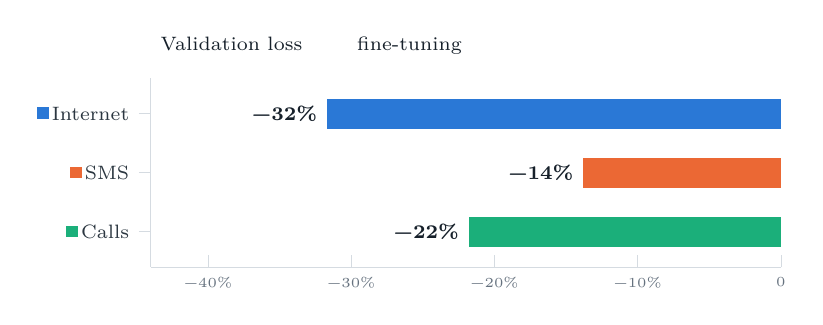
\begin{tikzpicture}
        \begin{axis}[deck, xbar, bar width=0.38cm, bar shift=0pt, width=0.66\linewidth, height=2.4cm, scale only axis,
            xmin=-44, xmax=0, ymin=0.4, ymax=3.6, ytick={1,2,3},
            yticklabels={\sCalls, \sSms, \sInet}, y tick label style={font=\scriptsize, text=text},
            xtick={-40,-30,-20,-10,0}, xticklabels={−40\%, −30\%, −20\%, −10\%, 0},
            nodes near coords, nodes near coords style={font=\scriptsize\bfseries, text=ink, anchor=east},
            point meta=explicit symbolic,
            title={Validation loss μετά το fine-tuning}]
          \addplot[fill=inet, draw=none] coordinates {(-31.7,3) [−32\%]};
          \addplot[fill=sms, draw=none] coordinates {(-13.8,2) [−14\%]};
          \addplot[fill=calls, draw=none] coordinates {(-21.8,1) [−22\%]};
        \end{axis}
      \end{tikzpicture}
      \figcap{Σε σχέση με το zero-shot, στις τελευταίες ημέρες του train.}
      \vspace{0.4em}

      \small Το validation διαλέγει το \alert{fine-tuned} ως εκπρόσωπο. Το zero-shot το κρατάμε για σύγκριση.
    \end{column}
  \end{columns}
\end{frame}
\note{Η εκφώνηση ζητά αποτελέσματα με και χωρίς fine-tuning, για τους δύο ορίζοντες. Στο zero-shot το μοντέλο δεν βλέπει καθόλου εκπαίδευση στα δεδομένα μας. Στο fine-tuning εκπαιδεύουμε τα δύο τελευταία από τα είκοσι στρώματα με την ίδια loss της προεκπαίδευσης, σε τυχαία παράθυρα του train, και κρατάμε τα βάρη με το μικρότερο validation loss. Το fine-tuning μειώνει το σφάλμα του validation σε όλες τις σειρές, οπότε εκπρόσωπος της οικογένειας είναι το fine-tuned. Όπως και στο LSTM όμως, το validation είναι κανονικές μέρες.}

% #####################################################################
\section{Αποτελέσματα}
% #####################################################################

\begin{frame}{Τέσσερις μετρικές, και τι λέει η καθεμία}
  \begin{columns}[T, onlytextwidth]
    \begin{column}{0.5\textwidth}
      \small
      Με $e_t = y_t - \hat y_t$ στα $n$ σημεία του test:
      \[
        \text{RMSE} = \sqrt{\tfrac1n \textstyle\sum_t e_t^2}, \qquad
        \text{MAE} = \tfrac1n \textstyle\sum_t |e_t|
      \]
      \[
        \text{MAPE} = \tfrac{100}{n} \textstyle\sum_t \left|\dfrac{e_t}{y_t}\right|
      \]
      \[
        \text{MASE} = \frac{\tfrac1n \sum_t |e_t|}{\tfrac{1}{n_{\text{tr}} - 144} \sum_{t} |y_t - y_{t-144}|}
      \]
      \figcap{Ο παρονομαστής: το σφάλμα του «όπως χθες» στο train.}
    \end{column}
    \begin{column}{0.47\textwidth}
      \small
      \begin{itemize}
        \item \textbf{RMSE, MAE}: στις μονάδες της σειράς, που εδώ \alert{δεν έχουν φυσική σημασία}. Το RMSE τιμωρεί περισσότερο τις αιχμές.
        \item \textbf{MAPE}: σχετικό σφάλμα, αλλά \alert{εκρήγνυται} τη νύχτα, όταν $y_t \to 0$ στα SMS και Calls.
        \item \textbf{MASE}: πόσο από το σφάλμα του «όπως χθες» κάνουμε. Το $0{,}3$ σημαίνει 30\%.
      \end{itemize}
      \vspace{0.3em}
      \begin{block}{Γιατί MASE}
        Δεν εξαρτάται από την κλίμακα ούτε από την κρυφή σταθερά, δεν εκρήγνυται, και \alert{συγκρίνει σειρές} μεταξύ τους.
      \end{block}
    \end{column}
  \end{columns}
\end{frame}
\note{Τα RMSE και MAE είναι στις μονάδες της σειράς, αλλά οι τιμές είναι κλιμακωμένες με άγνωστη σταθερά, οπότε ερμηνεύονται μόνο σχετικά: ένα MAE 29 όταν η κορυφή είναι γύρω στο 1200 είναι περίπου 2\% της κορυφής. Το RMSE δίνει μεγαλύτερο βάρος στα μεγάλα σφάλματα. Η MAPE αποτυγχάνει εδώ: στα Calls υπάρχουν εκατοντάδες δεκάλεπτα με τιμή κάτω από 1, όπου η MAPE φτάνει τις δεκάδες χιλιάδες τοις εκατό, οπότε ένα σφάλμα 2 μονάδων στις 4 το πρωί μετράει όσο εκατοντάδες σφάλματα το μεσημέρι. Στο Internet, που δεν πλησιάζει ποτέ το μηδέν, είναι αξιόπιστη. Η MASE διαιρεί το MAE με μία σταθερά, το σφάλμα του κανόνα «όπως χθες» στο train. Η σταθερά της ανωνυμοποίησης απλοποιείται, δεν εκρήγνυται τη νύχτα, είναι συμμετρική, και επιτρέπει να συγκρίνουμε Internet με SMS με έναν αριθμό. Γι' αυτό είναι η κύρια μετρική μας. Όλες οι μετρικές είναι στις εφεδρικές διαφάνειες.}

% =====================================================================
\begin{frame}{Το TimesFM έχει το μικρότερο σφάλμα παντού}
  \centering
  \footnotesize
  \begin{tabular}{@{}lcccccc@{}}
    \toprule
    & \multicolumn{2}{c}{\sInet} & \multicolumn{2}{c}{\sSms} & \multicolumn{2}{c}{\sCalls} \\
    \cmidrule(lr){2-3}\cmidrule(lr){4-5}\cmidrule(l){6-7}
    MASE & 10\,λεπ. & 50\,λεπ. & 10\,λεπ. & 50\,λεπ. & 10\,λεπ. & 50\,λεπ. \\
    \midrule
    \muted{Seasonal naive} & \muted{1,136} & \muted{1,122} & \muted{1,496} & \muted{1,463} & \muted{1,459} & \muted{1,447} \\
    Naive               & 0,302 & 0,480 & 0,602 & 0,759 & 0,438 & 0,599 \\
    ARIMA-x             & 0,296 & 0,433 & 0,580 & 0,724 & 0,410 & 0,520 \\
    LSTM                & 0,409 & 0,592 & 0,646 & 0,791 & 0,496 & 0,578 \\
    TimesFM fine-tuned  & \alert{0,249} & \alert{0,350} & \alert{0,536} & \alert{0,645} & \alert{0,366} & \alert{0,436} \\
    \midrule
    \muted{TimesFM zero-shot} & \muted{0,238} & \muted{0,313} & \muted{0,522} & \muted{0,618} & \muted{0,361} & \muted{0,419} \\
    \bottomrule
  \end{tabular}

  \vspace{0.5em}
  \raggedright\small
  \begin{itemize}
    \item Πρώτο σε κάθε σειρά, ορίζοντα και μετρική (εκτός MAPE). Η zero-shot εκδοχή, \alert{χωρίς καμία εκπαίδευση}, είναι ακόμη λίγο καλύτερη.
    \item Το ARIMA-x είναι λίγο καλύτερο από το Naive. Το LSTM του validation είναι \alert{χειρότερο από το Naive} σε 5 από τις 6 στήλες.
    \item Η δυσκολία είναι ίδια για όλα: Internet < Calls < SMS.
  \end{itemize}
\end{frame}
\note{Στον πίνακα η MASE στο test για τους εκπροσώπους. Η seasonal naive είναι παντού τελευταία, πάνω από 1, γιατί ο κανόνας «όπως χθες» αποτυγχάνει στις γιορτές και στη μετάβαση προς το Σαββατοκύριακο. Το TimesFM fine-tuned είναι πρώτο σε όλες τις στήλες, και η zero-shot εκδοχή, στην τελευταία γραμμή, είναι ακόμη καλύτερη: το fine-tuning βοήθησε στο validation αλλά όχι στο test. Το LSTM εδώ είναι 9 έως 38\% χειρότερο από το ARIMA-x, το αντίθετο από το 84 έως 87\% υπέρ του LSTM στο άρθρο των Siami-Namini. Οι σειρές μας είναι κυρίως γραμμικές και περιοδικές, ενώ οι οικονομικές σειρές του άρθρου έχουν τάσεις· το ARIMA-x ξέρει επιπλέον το ημερολόγιο και ξαναεκτιμάται σε κάθε βήμα· και το test μας έχει γιορτές. Τα SMS είναι τα δυσκολότερα, λόγω των απρόβλεπτων αιχμών.}

% =====================================================================
\begin{frame}{Πότε μια πρόβλεψη «πετυχαίνει»: όταν νικά καθαρά τον απλό κανόνα}
  \centering
  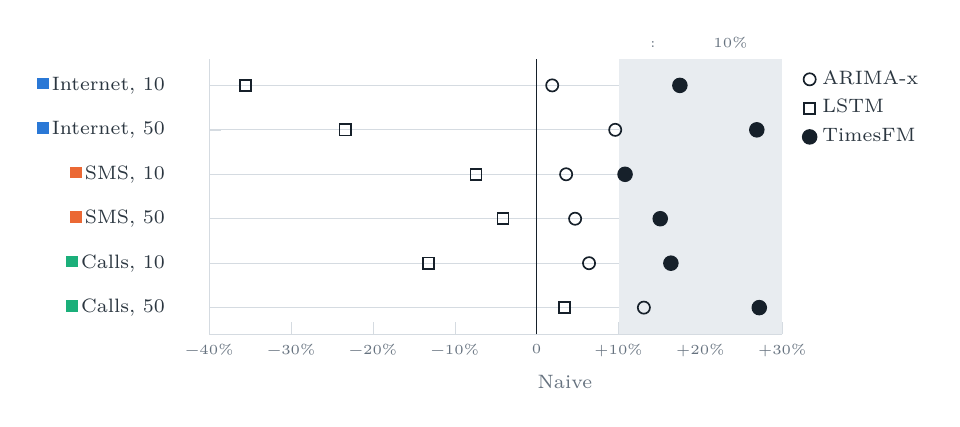
\begin{tikzpicture}
    \begin{axis}[deck, width=0.6\textwidth, height=3.5cm, scale only axis,
        xmin=-40, xmax=30, ymin=0.4, ymax=6.6,
        xtick={-40,-30,-20,-10,0,10,20,30}, xticklabels={−40\%, −30\%, −20\%, −10\%, 0, +10\%, +20\%, +30\%},
        ytick={1,...,6}, y tick label style={font=\scriptsize, text=text},
        yticklabels={{\ser{calls}{Calls}, 50 λεπτά}, {\ser{calls}{Calls}, 10 λεπτά},
                     {\ser{sms}{SMS}, 50 λεπτά}, {\ser{sms}{SMS}, 10 λεπτά},
                     {\ser{inet}{Internet}, 50 λεπτά}, {\ser{inet}{Internet}, 10 λεπτά}},
        xlabel={μικρότερο σφάλμα από το Naive},
        ymajorgrids, major grid style={draw=rule, line width=0.3pt},
        legend style={at={(1.02,1)}, anchor=north west}, legend cell align=left, clip=false]
      \fill[fillc] (axis cs:10,0.4) rectangle (axis cs:30,6.6);
      \node[anchor=south west, font=\tiny, text=muted, inner xsep=0pt] at (axis cs:10,6.62) {επιτυχία: τουλάχιστον 10\%};
      \draw[ink, line width=0.5pt] (axis cs:0,0.4) -- (axis cs:0,6.6);
      \addplot[only marks, mark=o, mark size=2.2pt, draw=ink, line width=0.6pt]
        coordinates {(1.9,6) (9.6,5) (3.6,4) (4.7,3) (6.4,2) (13.1,1)};
      \addlegendentry{ARIMA-x}
      \addplot[only marks, mark=square, mark size=2pt, draw=ink, line width=0.6pt]
        coordinates {(-35.6,6) (-23.4,5) (-7.4,4) (-4.1,3) (-13.2,2) (3.4,1)};
      \addlegendentry{LSTM}
      \addplot[only marks, mark=*, mark size=2.6pt, fill=ink, draw=ink]
        coordinates {(17.5,6) (26.9,5) (10.8,4) (15.1,3) (16.4,2) (27.2,1)};
      \addlegendentry{TimesFM}
    \end{axis}
  \end{tikzpicture}

  \vspace{0.3em}
  \raggedright\small
  \begin{columns}[T, onlytextwidth]
    \begin{column}{0.32\textwidth}
      \textbf{MASE < 1}: πολύ χαλαρό, το περνά ακόμη και το Naive.
    \end{column}
    \begin{column}{0.32\textwidth}
      \textbf{Έναντι του Naive}: το πραγματικό κατώφλι, γιατί το Naive δεν κοστίζει τίποτα.
    \end{column}
    \begin{column}{0.32\textwidth}
      \textbf{Έναντι του περιθωρίου}: σφάλμα μικρότερο από τη χωρητικότητα που κρατά ο πάροχος.
    \end{column}
  \end{columns}
\end{frame}
\note{Η εκφώνηση ρωτά πώς θα κρίναμε αν η πρόβλεψη πέτυχε. Μια μετρική μόνη της δεν το λέει. Η MASE κάτω από 1 είναι πολύ χαλαρό κριτήριο, γιατί σε δέκα λεπτά η τελευταία τιμή είναι πολύ καλύτερη πρόβλεψη από την τιμή χθες. Το πραγματικό κατώφλι είναι η βελτίωση έναντι του Naive. Ορίσαμε επιτυχία ως τουλάχιστον 10\% μικρότερο σφάλμα· το όριο είναι δική μας επιλογή, και φαίνεται ως η σκιασμένη ζώνη. Το TimesFM είναι μέσα στη ζώνη σε κάθε γραμμή. Το ARIMA-x είναι πάντα πάνω από το μηδέν αλλά μπαίνει στη ζώνη μόνο στα Calls για 50 λεπτά. Το LSTM του validation είναι κάτω από το Naive παντού εκτός από εκεί. Το τρίτο κριτήριο είναι τηλεπικοινωνιακό: στο Internet το TimesFM έχει σχετικό σφάλμα 8 έως 12\%, κάτω από το συνηθισμένο περιθώριο χωρητικότητας 15 έως 30\%.}

% =====================================================================
\begin{frame}{Όλα πιάνουν το σχήμα, κανένα την αιχμή της Πρωτοχρονιάς}
  \begin{columns}[T, onlytextwidth]
    \begin{column}{0.64\textwidth}
      \IfFileExists{figs/forecast_holidays.dat}{%
        \begin{tikzpicture}
          \begin{groupplot}[deck, group style={group size=1 by 2, vertical sep=0.45cm, xticklabels at=edge bottom},
              width=0.9\linewidth, height=1.9cm, scale only axis, xmin=0, xmax=9, ymin=0,
              xtick={0,...,8}, xticklabels={24/12,25/12,26/12,27/12,28/12,29/12,30/12,31/12,1/1},
              legend style={at={(0,-0.38)}, anchor=north west, legend columns=4}, unbounded coords=jump]
            \nextgroupplot[ymax=2100, title={\sInet}]
              \addplot[quiet, line width=0.4pt, dotted] table[x=x, y=inet_arima] {figs/forecast_holidays.dat};
              \addplot[quiet, line width=0.4pt, dashed] table[x=x, y=inet_lstm] {figs/forecast_holidays.dat};
              \addplot[ink, line width=0.5pt] table[x=x, y=inet_tfm] {figs/forecast_holidays.dat};
              \addplot[inet, line width=1pt, opacity=0.85] table[x=x, y=inet_actual] {figs/forecast_holidays.dat};
            \nextgroupplot[ymax=1650, title={\sSms}]
              \addplot[quiet, line width=0.4pt, dotted] table[x=x, y=sms_arima] {figs/forecast_holidays.dat};
              \addlegendentry{ARIMA-x}
              \addplot[quiet, line width=0.4pt, dashed] table[x=x, y=sms_lstm] {figs/forecast_holidays.dat};
              \addlegendentry{LSTM}
              \addplot[ink, line width=0.5pt] table[x=x, y=sms_tfm] {figs/forecast_holidays.dat};
              \addlegendentry{TimesFM}
              \addplot[sms, line width=1pt, opacity=0.85] table[x=x, y=sms_actual] {figs/forecast_holidays.dat};
              \addlegendentry{πραγματική τιμή}
          \end{groupplot}
        \end{tikzpicture}
        \figcap{24/12 έως 01/01, πρόβλεψη 50 λεπτών.}%
      }{%
        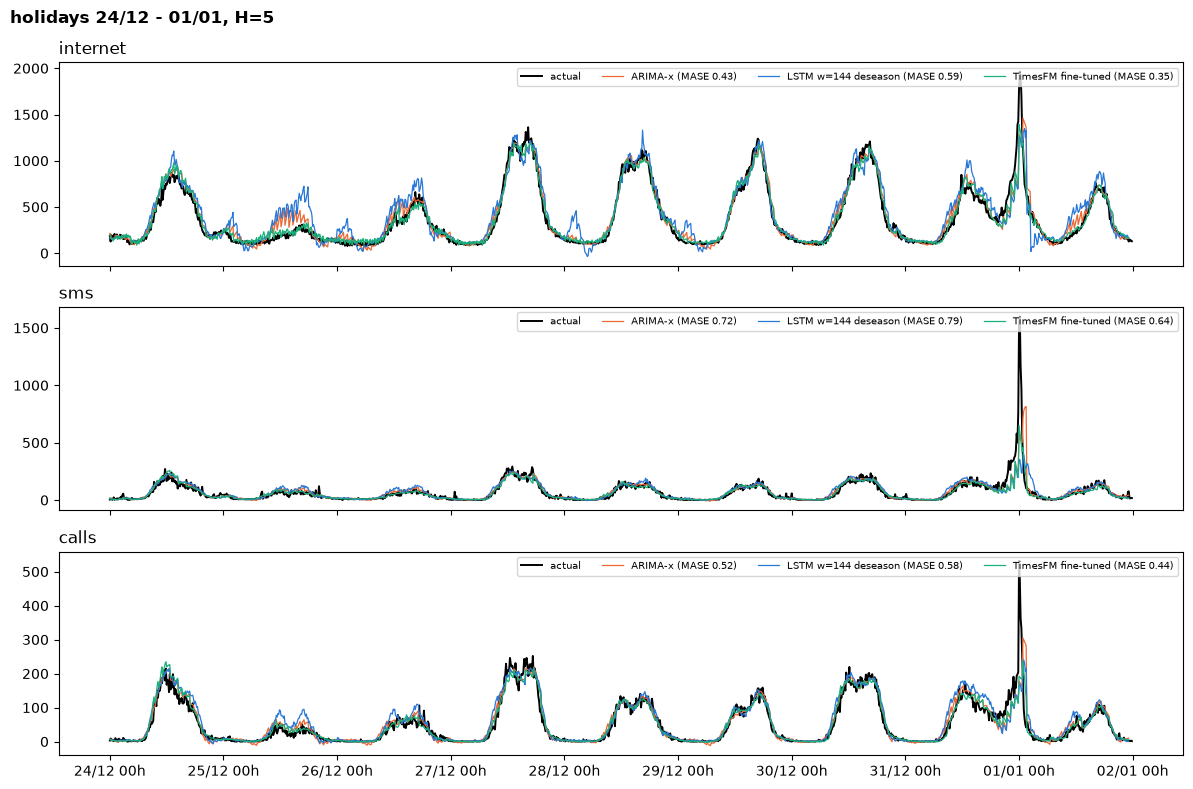
\includegraphics[width=\linewidth, height=0.66\textheight, keepaspectratio]{forecast_holidays.png}
        \figcap{24/12 έως 01/01, πρόβλεψη 50 λεπτών. Μαύρο: πραγματική τιμή. Πορτοκαλί: ARIMA-x, μπλε: LSTM, πράσινο: TimesFM.}%
      }
    \end{column}
    \begin{column}{0.33\textwidth}
      \small
      \begin{itemize}
        \item Το ημερήσιο σχήμα το πιάνουν \alert{όλα}.
        \item 25–26/12: τα μοντέλα του train περιμένουν κανονική μέρα και \alert{υπερεκτιμούν}. Το TimesFM προσαρμόζεται πιο γρήγορα.
        \item Την αιχμή της Πρωτοχρονιάς \alert{δεν την προβλέπει κανείς}· φαίνεται με καθυστέρηση.
      \end{itemize}
    \end{column}
  \end{columns}
\end{frame}
\note{Η εκφώνηση ζητά απεικονίσεις της πραγματικής σειράς μαζί με την πρόβλεψη. Στις κανονικές μέρες οι προβλέψεις σχεδόν καλύπτουν την πραγματική σειρά, και οι διαφορές αφορούν το ύψος της κορυφής. Τη νύχτα το σφάλμα είναι πολύ μικρό· τα μεγάλα σφάλματα είναι στις ώρες κίνησης, όπου ένα λάθος προκαλεί συμφόρηση. Εδώ δείχνουμε τις γιορτές, όπου φαίνονται οι διαφορές. Τα μοντέλα του train υπερεκτιμούν τα Χριστούγεννα. Την αιχμή της Πρωτοχρονιάς, περίπου 70 φορές τα κανονικά SMS σε δέκα λεπτά, δεν την προβλέπει κανένα μοντέλο από το ιστορικό· εμφανίζεται στην πρόβλεψη ένα βήμα αργότερα. Για τέτοια γεγονότα χρειάζεται ημερολόγιο εκδηλώσεων.}

% =====================================================================
\begin{frame}{Ό,τι βοήθησε στο validation, έβλαψε στις γιορτές}
  \begin{columns}[T, onlytextwidth]
    \begin{column}{0.6\textwidth}
      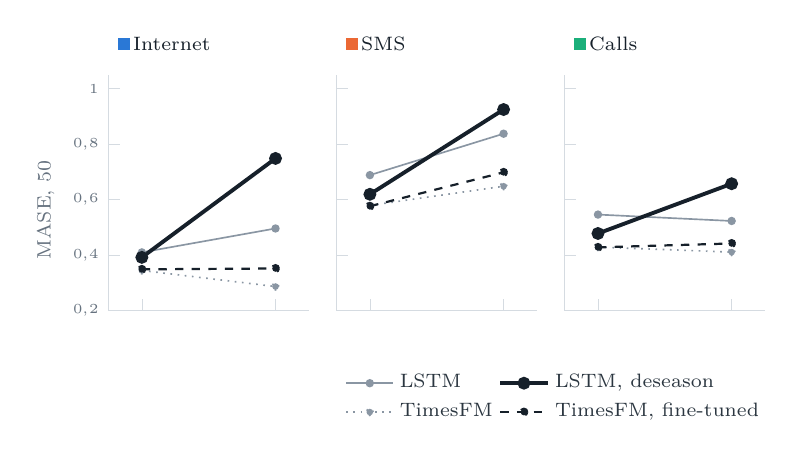
\begin{tikzpicture}
        \begin{groupplot}[deck, group style={group size=3 by 1, horizontal sep=0.35cm, yticklabels at=edge left},
            width=0.21\textwidth, height=3.0cm, scale only axis, xmin=-0.25, xmax=1.25, ymin=0.2, ymax=1.05,
            xtick={0,1}, xticklabels={κανονικές, γιορτές}, ytick={0.2,0.4,0.6,0.8,1},
            yticklabel style={/pgf/number format/use comma, /pgf/number format/fixed},
            legend style={at={(0,-0.22)}, anchor=north west, legend columns=2}, legend cell align=left]
          \nextgroupplot[title={\sInet}, ylabel={MASE, 50 λεπτά}]
            \addplot[quiet, line width=0.6pt, mark=*, mark size=1.2pt] coordinates {(0,0.410) (1,0.496)};
            \addplot[ink, line width=1.4pt, mark=*, mark size=1.6pt] coordinates {(0,0.392) (1,0.748)};
            \addplot[quiet, line width=0.6pt, dotted, mark=*, mark size=1.2pt] coordinates {(0,0.345) (1,0.287)};
            \addplot[ink, line width=0.8pt, dashed, mark=*, mark size=1.2pt] coordinates {(0,0.349) (1,0.352)};
          \nextgroupplot[title={\sSms}]
            \addplot[quiet, line width=0.6pt, mark=*, mark size=1.2pt] coordinates {(0,0.688) (1,0.837)};
            \addlegendentry{LSTM}
            \addplot[ink, line width=1.4pt, mark=*, mark size=1.6pt] coordinates {(0,0.619) (1,0.924)};
            \addlegendentry{LSTM, deseason}
            \addplot[quiet, line width=0.6pt, dotted, mark=*, mark size=1.2pt] coordinates {(0,0.579) (1,0.648)};
            \addlegendentry{TimesFM}
            \addplot[ink, line width=0.8pt, dashed, mark=*, mark size=1.2pt] coordinates {(0,0.576) (1,0.698)};
            \addlegendentry{TimesFM, fine-tuned}
          \nextgroupplot[title={\sCalls}]
            \addplot[quiet, line width=0.6pt, mark=*, mark size=1.2pt] coordinates {(0,0.546) (1,0.523)};
            \addplot[ink, line width=1.4pt, mark=*, mark size=1.6pt] coordinates {(0,0.478) (1,0.657)};
            \addplot[quiet, line width=0.6pt, dotted, mark=*, mark size=1.2pt] coordinates {(0,0.429) (1,0.411)};
            \addplot[ink, line width=0.8pt, dashed, mark=*, mark size=1.2pt] coordinates {(0,0.428) (1,0.442)};
        \end{groupplot}
      \end{tikzpicture}
      \figcap{Κανονικές: 17–23/12. Γιορτές: 24/12–01/01. Μικρότερο είναι καλύτερο.}
    \end{column}
    \begin{column}{0.37\textwidth}
      \small
      \begin{itemize}
        \item Η από-περιοδικοποίηση βοηθά στις κανονικές μέρες, αλλά στις γιορτές το σφάλμα \alert{εκτινάσσεται}: το $S_t$ περιμένει κανονική μέρα.
        \item Το fine-tuning δεν αλλάζει τις κανονικές μέρες και \alert{χειροτερεύει τις γιορτές}.
        \item Ταιριάζει καλύτερα στο παρελθόν $\neq$ προβλέπει καλύτερα ένα μέλλον που αλλάζει.
      \end{itemize}
    \end{column}
  \end{columns}
\end{frame}
\note{Η εκφώνηση ρωτά αν η από-περιοδικοποίηση βοηθά. Η απάντηση είναι: εξαρτάται από το αν το μέλλον μοιάζει με το παρελθόν. Χωρίζουμε το test σε κανονικές μέρες και γιορτές. Οι σκούρες γραμμές είναι τα δύο κόλπα που βελτίωσαν το validation. Η από-περιοδικοποίηση, η παχιά γραμμή, ανεβαίνει απότομα στις γιορτές σε κάθε σειρά, κατά 40 έως 90\%. Στο test η τυπική απόκλιση του υπολοίπου είναι δύο έως τρεισήμισι φορές μεγαλύτερη από το train, οπότε ένα μοντέλο που περιμένει κανονική μέρα κάνει μεγάλα λάθη. Το απλό LSTM και το TimesFM zero-shot ακολουθούν το πρόσφατο επίπεδο και αντέχουν καλύτερα. Και οι δύο σκούρες γραμμές είναι οι εκπρόσωποι που διάλεξε το validation: το test δείχνει το κόστος αυτής της επιλογής, που δεν μπορούσαμε να το δούμε από πριν.}

% =====================================================================
\begin{frame}{Διαστήματα 95\%: του TimesFM ακολουθούν την ώρα}
  \begin{columns}[T, onlytextwidth]
    \begin{column}{0.6\textwidth}
      \IfFileExists{figs/intervals.dat}{%
        \begin{tikzpicture}
          \begin{groupplot}[deck, group style={group size=1 by 2, vertical sep=0.5cm, xticklabels at=edge bottom},
              width=0.92\linewidth, height=1.75cm, scale only axis, xmin=0, xmax=2, ymin=-150, ymax=1800,
              xtick={0,0.5,1,1.5,2}, xticklabels={18/12, 12:00, 19/12, 12:00, 20/12}, ytick={0,500,1000,1500}]
            \nextgroupplot[title={ARIMA-x, \sInet}]
              \addplot[name path=hi, draw=none, forget plot] table[x=x, y=arima_hi] {figs/intervals.dat};
              \addplot[name path=lo, draw=none, forget plot] table[x=x, y=arima_lo] {figs/intervals.dat};
              \addplot[fillc, forget plot] fill between[of=hi and lo];
              \draw[rule] (axis cs:0,0) -- (axis cs:2,0);
              \addplot[inet, line width=0.6pt] table[x=x, y=actual] {figs/intervals.dat};
            \nextgroupplot[title={TimesFM fine-tuned, \sInet}]
              \addplot[name path=hi, draw=none, forget plot] table[x=x, y=tfm_hi] {figs/intervals.dat};
              \addplot[name path=lo, draw=none, forget plot] table[x=x, y=tfm_lo] {figs/intervals.dat};
              \addplot[fillc, forget plot] fill between[of=hi and lo];
              \draw[rule] (axis cs:0,0) -- (axis cs:2,0);
              \addplot[inet, line width=0.6pt] table[x=x, y=actual] {figs/intervals.dat};
          \end{groupplot}
        \end{tikzpicture}
        \figcap{Short-term, δύο εργάσιμες. Γκρι: το διάστημα 95\%. Μπλε: η πραγματική τιμή.}%
      }{%
        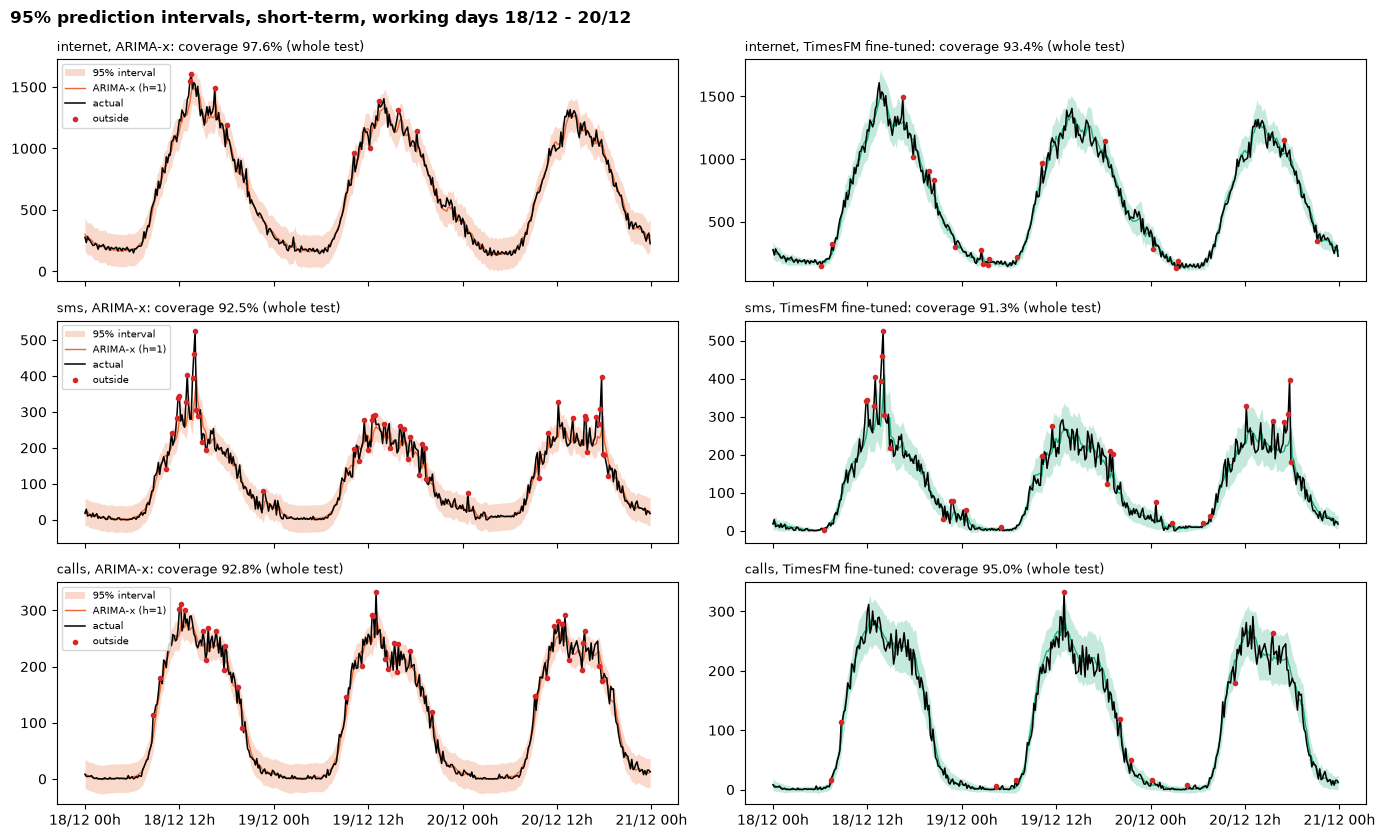
\includegraphics[width=\linewidth, height=0.7\textheight, keepaspectratio]{intervals.png}
        \figcap{Short-term, εργάσιμες 18–20/12. Αριστερά ARIMA-x, δεξιά TimesFM fine-tuned. Κόκκινα: σημεία εκτός.}%
      }
    \end{column}
    \begin{column}{0.37\textwidth}
      \footnotesize
      \begin{tabular}{@{}lccc@{}}
        \toprule
        & \sInet & \sSms & \sCalls \\
        \midrule
        \multicolumn{4}{@{}l}{\muted{κάλυψη (στόχος 95\%)}} \\
        ARIMA-x & 98\% & 92\% & 93\% \\
        TimesFM & 93\% & 91\% & 95\% \\
        \midrule
        \multicolumn{4}{@{}l}{\muted{μέσο πλάτος, σχετικά}} \\
        ARIMA-x & 2,08 & 2,91 & 2,29 \\
        TimesFM & \alert{1,20} & \alert{2,19} & \alert{1,79} \\
        \bottomrule
      \end{tabular}
      \vspace{0.5em}

      \small
      \begin{itemize}
        \item ARIMA-x: \alert{σταθερό πλάτος}, πολύ φαρδύ τη νύχτα (κάτω από το μηδέν), στενό στην αιχμή.
        \item TimesFM: \alert{στενότερο} και προσαρμόζεται στην ώρα, με κάλυψη κοντά στο 95\%.
      \end{itemize}
    \end{column}
  \end{columns}
\end{frame}
\note{Αυτό είναι το bonus της εκφώνησης: διαστήματα πρόβλεψης 95\% για το short-term, για το ARIMA-x και το TimesFM. Για το ARIMA-x το διάστημα είναι η πρόβλεψη συν πλην 1,96 σίγμα, με το σίγμα του fit· είναι πρακτικά ίδιο όλη την ημέρα, οπότε τη νύχτα πηγαίνει και κάτω από το μηδέν και στην αιχμή είναι πολύ στενό, όπως προέβλεπαν τα κατάλοιπα. Για το TimesFM το βγάζουμε από τα ποσοστημόρια 10\% και 90\%, θεωρώντας κανονική κατανομή γύρω από τη διάμεσο, οπότε αλλάζει σε κάθε σημείο. Η κάλυψη, το ποσοστό των σημείων του test μέσα στο διάστημα, είναι κοντά στο 95\% και για τα δύο, αλλά του TimesFM είναι 20 έως 40\% στενότερο. Τα σημεία εκτός είναι κυρίως από πάνω, γιατί τις ανοδικές αιχμές δεν τις προβλέπει κανείς· η υποκάλυψη θα μπορούσε να διορθωθεί με conformal prediction. Τηλεπικοινωνιακά μετράει το άνω όριο: αν δεσμεύουμε χωρητικότητα ίση με αυτό, η ζήτηση την ξεπερνά περίπου στο 2,5\% των δεκαλέπτων.}

% #####################################################################
\section{Σε δίκτυο 6G}
% #####################################################################

\begin{frame}{Στο δίκτυο: η πρόβλεψη ως rApp στον κλειστό βρόχο}
  \centering
  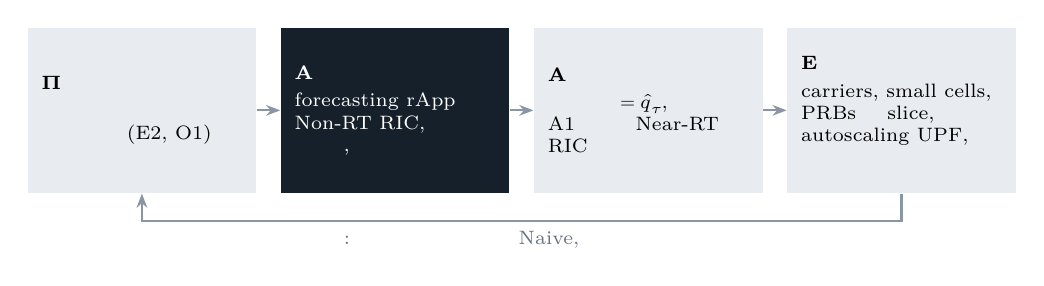
\begin{tikzpicture}[node distance=0.3cm, >={Stealth[length=1.8mm]},
      stage/.style={fill=fillc, text width=2.55cm, minimum height=2.1cm, align=flush left,
                   inner xsep=5pt, inner ysep=5pt, font=\scriptsize,
                   execute at begin node={\hyphenpenalty 10000\relax}},
      key/.style={stage, fill=ink, text=white}]
    \node[stage] (a) {\textbf{Παρακολούθηση}\\[2pt] φορτίο κάθε κυψέλης από τους σταθμούς βάσης (E2, O1)};
    \node[key, right=of a] (b) {\textbf{Ανάλυση}\\[2pt] forecasting rApp στον Non-RT RIC, κάθε δεκάλεπτο, με ποσοστημόρια};
    \node[stage, right=of b] (c) {\textbf{Απόφαση}\\[2pt] χωρητικότητα $= \hat q_\tau$, ως πολιτική A1 προς τον Near-RT RIC};
    \node[stage, right=of c] (d) {\textbf{Εκτέλεση}\\[2pt] carriers, small cells, PRBs ανά slice, autoscaling UPF, ύπνος τη νύχτα};
    \foreach \u/\v in {a/b, b/c, c/d} \draw[->, thick, quiet] (\u) -- (\v);
    \draw[->, thick, quiet] (d.south) -- ++(0,-0.35) -| (a.south)
      node[pos=0.25, below, font=\scriptsize, text=muted] {πραγματική τιμή: αν το μοντέλο χάνει από το Naive, εφεδρικό μοντέλο και επανεκπαίδευση};
  \end{tikzpicture}

  \vspace{1.3em}
  \raggedright\small
  \begin{columns}[T, onlytextwidth]
    \begin{column}{0.48\textwidth}
      \textbf{Ποιο ποσοστημόριο.} $\tau^* = \dfrac{c_{\text{under}}}{c_{\text{under}} + c_{\text{over}}}$: η υποεκτίμηση (συμφόρηση, SLA) κοστίζει περισσότερο από την υπερεκτίμηση (ενέργεια).
    \end{column}
    \begin{column}{0.48\textwidth}
      \textbf{Ανά slice.} Υψηλό $\tau$ για URLLC και φωνή, χαμηλότερο για eMBB. Τη νύχτα, χαμηλό σφάλμα: ο εξοπλισμός κλείνει με ασφάλεια.
    \end{column}
  \end{columns}
\end{frame}
\note{Πώς θα το ενορχηστρώναμε σε πραγματικό δίκτυο. Ακολουθούμε το ZSM και την αρχιτεκτονική O-RAN, όπου η ευφυΐα του RAN είναι σε δύο ελεγκτές: τον Non-RT RIC, με βρόχους πάνω από ένα δευτερόλεπτο, και τον Near-RT RIC, με βρόχους από δέκα χιλιοστά έως ένα δευτερόλεπτο. Οι μετρήσεις φορτίου ρέουν από τους σταθμούς βάσης. Ένα forecasting rApp τρέχει σε κάθε νέο δεκάλεπτο, ακριβώς το rolling σχήμα μας, και βγάζει πρόβλεψη με ποσοστημόρια. Η χωρητικότητα ορίζεται από ένα άνω ποσοστημόριο, που προκύπτει από το κόστος της υποεκτίμησης έναντι της υπερεκτίμησης, και περνά ως πολιτική στον Near-RT RIC. Μετά από κάθε δεκάλεπτο συγκρίνουμε με την πραγματική τιμή· αν το μοντέλο γίνει χειρότερο από το Naive για αρκετό διάστημα, όπως στις γιορτές, ο βρόχος γυρίζει σε ένα απλό εφεδρικό μοντέλο και ζητά επανεκπαίδευση.}

% =====================================================================
\begin{frame}{Χωράει η πρόβλεψη σε έναν κύκλο δέκα λεπτών;}
  \begin{columns}[T, onlytextwidth]
    \begin{column}{0.56\textwidth}
      \small
      \begin{tabular}{@{}lll@{}}
        \toprule
        & Εκπαίδευση & 10.000 κυψέλες \\
        \midrule
        ARIMA-x, νέο fit κάθε βήμα & \textasciitilde 11 s & \alert{\textasciitilde 4 ώρες} \\
        ARIMA-x, μόνο ενημέρωση & \textasciitilde 11 s & \textasciitilde 30 s \\
        LSTM & 4–17 λεπτά & < 1 s \\
        TimesFM & 0 ή \textasciitilde 27 λεπτά & \textasciitilde 8 λεπτά \\
        \bottomrule
      \end{tabular}
      \figcap{Μία πρόβλεψη πέντε βημάτων ανά κυψέλη. CPU χωρίς GPU, ένας server.}
    \end{column}
    \begin{column}{0.4\textwidth}
      \small
      \begin{itemize}
        \item Για μία κυψέλη \alert{όλα} χωράνε άνετα.
        \item Σε μεγάλο δίκτυο το TimesFM χωράει \alert{χωρίς περιθώριο} σε CPU· με GPU πολύ πιο άνετα.
        \item Για βρόχους κάτω του δευτερολέπτου (Near-RT RIC) μόνο ελαφριά μοντέλα.
      \end{itemize}
    \end{column}
  \end{columns}
  \vspace{0.8em}
  \begin{block}{Πρόταση}
    \alert{TimesFM} σε GPU στον Non-RT RIC για προβλέψεις λεπτών. \alert{LSTM ή ARIMA-x} στον Near-RT RIC για γρήγορες διορθώσεις και ως εφεδρικά. Το zero-shot δεν θέλει εκπαίδευση ανά κυψέλη, άρα καλύπτει και νέες κυψέλες.
  \end{block}
\end{frame}
\note{Η εκφώνηση ρωτά αν οι χρόνοι inference ευνοούν μια online διαδικασία. Μετρήσαμε στον ίδιο server, σε CPU. Το ARIMA-x με νέο fit σε κάθε βήμα κοστίζει περίπου 1,4 δευτερόλεπτα ανά πρόβλεψη, οπότε σε δέκα χιλιάδες κυψέλες θέλει ώρες. Αν όμως κάνουμε το fit offline, π.χ. μία φορά την ημέρα, και σε κάθε βήμα μόνο ενημερώνουμε την κατάσταση με τη νέα τιμή, κοστίζει λίγα χιλιοστά. Το LSTM είναι κάτω από ένα χιλιοστό ανά πρόβλεψη. Το TimesFM θέλει περίπου 48 χιλιοστά ανά πρόβλεψη σε batch, οπότε ένας κύκλος δέκα χιλιάδων κυψελών κρατά περίπου 8 λεπτά: χωράει, αλλά χωρίς περιθώριο. Γι' αυτό προτείνουμε ιεραρχική αρχιτεκτονική: το ακριβό αλλά ακριβέστερο μοντέλο εκεί όπου ο βρόχος είναι λεπτών, και ελαφριά μοντέλα για τους γρήγορους βρόχους.}

% =====================================================================
\begin{frame}{Συμπεράσματα}
  \begin{enumerate}
    \item Στα 10 λεπτά η τελευταία τιμή είναι ήδη καλή πρόβλεψη. Ένα μοντέλο αξίζει μόνο αν \alert{νικά το Naive}.
    \vspace{0.5em}
    \item Τα τεστ και τα ACF/PACF οδηγούν σε ARIMA με τον κύκλο ως είσοδο. Το ARIMA-x νικά το Naive \alert{οριακά}.
    \vspace{0.5em}
    \item Το LSTM του validation δεν νικά το Naive σχεδόν πουθενά. Οι σειρές μας είναι κυρίως γραμμικές και περιοδικές.
    \vspace{0.5em}
    \item Το \alert{TimesFM} κερδίζει παντού, κατά 11–27\% έναντι του Naive, με στενότερα διαστήματα. Χωρίς fine-tuning κερδίζει ακόμη περισσότερο (13–35\%).
    \vspace{0.5em}
    \item Ό,τι βελτίωσε το validation δεν βοήθησε στις γιορτές: \alert{το μέλλον δεν μοιάζει πάντα με το παρελθόν}. Αιχμές όπως της Πρωτοχρονιάς θέλουν ημερολόγιο εκδηλώσεων.
  \end{enumerate}
\end{frame}
\note{Κλείνοντας: η persistence είναι ισχυρό σημείο αναφοράς στα δέκα λεπτά. Η κλασική διαδικασία Box-Jenkins δίνει ένα λογικό ARIMA, που όμως κερδίζει λίγο. Το LSTM δεν έδειξε εδώ το πλεονέκτημα του άρθρου. Το TimesFM κερδίζει παντού, και μάλιστα καλύτερα χωρίς εκπαίδευση, αλλά κοστίζει περισσότερο στο inference. Και η επιλογή με βάση το validation μπορεί να παραπλανήσει όταν το test περιέχει συνθήκες που δεν έχουμε δει. Ευχαριστούμε.}

% #####################################################################
\appendix
\section{Εφεδρικές}
% #####################################################################

\begin{frame}{Εφεδρική: όλες οι μετρικές, short-term (10 λεπτά)}
  \centering
  \footnotesize\setlength{\tabcolsep}{4.5pt}
  \begin{tabular}{@{}lccccccccc@{}}
    \toprule
    & \multicolumn{3}{c}{\sInet} & \multicolumn{3}{c}{\sSms} & \multicolumn{3}{c}{\sCalls} \\
    \cmidrule(lr){2-4}\cmidrule(lr){5-7}\cmidrule(l){8-10}
    & RMSE & MAE & MAPE & RMSE & MAE & MAPE & RMSE & MAE & MAPE \\
    \midrule
    Naive              & 51,8 & 36,9 & 10,1\% & 32,0 & 15,9 & \muted{336\%} & 16,7 & 9,8 & \muted{2.408\%} \\
    Seasonal naive     & 232,0 & 138,8 & 36,5\% & 88,6 & 39,7 & \muted{704\%} & 57,4 & 32,6 & \muted{2.362\%} \\
    ARIMA-x            & 52,5 & 36,2 & 10,7\% & 35,7 & 15,4 & \muted{321\%} & 16,1 & 9,2 & \muted{2.873\%} \\
    LSTM               & 72,6 & 50,0 & 16,5\% & 43,2 & 17,1 & \muted{535\%} & 19,2 & 11,1 & \muted{3.270\%} \\
    TimesFM fine-tuned & \alert{44,4} & \alert{30,5} & \alert{8,0\%} & \alert{31,3} & \alert{14,2} & \muted{479\%} & \alert{14,6} & \alert{8,2} & \muted{1.692\%} \\
    \bottomrule
  \end{tabular}

  \vspace{0.8em}
  \raggedright\small
  \begin{itemize}
    \item Η κατάταξη με RMSE και MAE είναι ίδια με της MASE.
    \item Στα SMS το ARIMA-x έχει μικρότερο MAE από το Naive αλλά \alert{μεγαλύτερο RMSE}: καλύτερο τις περισσότερες στιγμές, χειρότερο στις αιχμές.
    \item Η MAPE στα SMS και Calls είναι γκρι: εκρήγνυται στις νυχτερινές τιμές κοντά στο μηδέν.
  \end{itemize}
\end{frame}
\note{Αν ρωτηθούμε για τις άλλες μετρικές. Τα RMSE και MAE είναι στις κλιμακωμένες μονάδες της σειράς, οπότε συγκρίνονται μόνο μέσα στην ίδια σειρά. Ο λόγος RMSE προς MAE είναι γύρω στο 1,25 για κανονικά σφάλματα· στα SMS φτάνει από 2 έως σχεδόν 3, γιατί λίγες απότομες αιχμές δίνουν πολύ μεγάλα σφάλματα.}

% =====================================================================
\begin{frame}{Εφεδρική: όλες οι μετρικές, long-term (50 λεπτά)}
  \centering
  \footnotesize\setlength{\tabcolsep}{4.5pt}
  \begin{tabular}{@{}lccccccccc@{}}
    \toprule
    & \multicolumn{3}{c}{\sInet} & \multicolumn{3}{c}{\sSms} & \multicolumn{3}{c}{\sCalls} \\
    \cmidrule(lr){2-4}\cmidrule(lr){5-7}\cmidrule(l){8-10}
    & RMSE & MAE & MAPE & RMSE & MAE & MAPE & RMSE & MAE & MAPE \\
    \midrule
    Naive              & 87,5 & 58,6 & 14,5\% & 43,0 & 20,1 & \muted{518\%} & 23,7 & 13,4 & \muted{1.637\%} \\
    Seasonal naive     & 227,3 & 137,1 & 35,1\% & 85,5 & 38,8 & \muted{699\%} & 56,9 & 32,3 & \muted{2.347\%} \\
    ARIMA-x            & 82,3 & 53,0 & 16,4\% & 52,9 & 19,2 & \muted{374\%} & 21,7 & 11,6 & \muted{3.588\%} \\
    LSTM               & 109,2 & 72,3 & 24,6\% & 55,6 & 21,0 & \muted{505\%} & 23,1 & 12,9 & \muted{3.297\%} \\
    TimesFM fine-tuned & \alert{65,7} & \alert{42,8} & \alert{11,7\%} & 44,5 & \alert{17,1} & \muted{513\%} & \alert{18,5} & \alert{9,7} & \muted{1.959\%} \\
    \bottomrule
  \end{tabular}

  \vspace{0.8em}
  \raggedright\small
  \begin{itemize}
    \item Στο Internet το TimesFM κάνει λάθος περίπου στο \alert{12\%} κάθε τιμής, κάτω από το συνηθισμένο περιθώριο χωρητικότητας.
    \item Στα SMS το Naive έχει οριακά μικρότερο RMSE από το TimesFM, λόγω των αιχμών.
  \end{itemize}
\end{frame}
\note{Ίδια εικόνα για τα πενήντα λεπτά. Το προβάδισμα του TimesFM μεγαλώνει, γιατί η τελευταία τιμή χάνει γρηγορότερα την αξία της όσο απομακρυνόμαστε.}

\end{document}
